% This is the Reed College LaTeX thesis template. Most of the work
% for the document class was done by Sam Noble (SN), as well as this
% template. Later comments etc. by Ben Salzberg (BTS). Additional
% restructuring and APA support by Jess Youngberg (JY).
% Your comments and suggestions are more than welcome; please email
% them to cus@reed.edu
%
% See http://web.reed.edu/cis/help/latex.html for help. There are a
% great bunch of help pages there, with notes on
% getting started, bibtex, etc. Go there and read it if you're not
% already familiar with LaTeX.
%
% Any line that starts with a percent symbol is a comment.
% They won't show up in the document, and are useful for notes
% to yourself and explaining commands.
% Commenting also removes a line from the document;
% very handy for troubleshooting problems. -BTS

% As far as I know, this follows the requirements laid out in
% the 2002-2003 Senior Handbook. Ask a librarian to check the
% document before binding. -SN

%%
%% Preamble
%%
% \documentclass{<something>} must begin each LaTeX document
\documentclass[12pt,twoside]{reedthesis}
% Packages are extensions to the basic LaTeX functions. Whatever you
% want to typeset, there is probably a package out there for it.
% Chemistry (chemtex), screenplays, you name it.
% Check out CTAN to see: http://www.ctan.org/
%%
\usepackage{graphicx,latexsym}
\usepackage{amsmath}
\usepackage{amssymb,amsthm}
\usepackage{longtable,booktabs,setspace}
\usepackage{chemarr} %% Useful for one reaction arrow, useless if you're not a chem major
\usepackage[hyphens]{url}
% Added by CII
\usepackage{hyperref}
\usepackage{lmodern}
% End of CII addition
\usepackage{rotating}

% Next line commented out by CII
%%% \usepackage{natbib}
% Comment out the natbib line above and uncomment the following two lines to use the new 
% biblatex-chicago style, for Chicago A. Also make some changes at the end where the 
% bibliography is included. 
%\usepackage{biblatex-chicago}
%\bibliography{thesis}


% Added by CII (Thanks, Hadley!)
% Use ref for internal links
\renewcommand{\hyperref}[2][???]{\autoref{#1}}
\def\chapterautorefname{Chapter}
\def\sectionautorefname{Section}
\def\subsectionautorefname{Subsection}
% End of CII addition

% Added by CII 
\usepackage{caption}
\captionsetup{width=5in}
% End of CII addition

% \usepackage{times} % other fonts are available like times, bookman, charter, palatino


% To pass between YAML and LaTeX the dollar signs are added by CII
\title{Enzymatic Promiscuity}
\author{Nelly Selem}
% The month and year that you submit your FINAL draft TO THE LIBRARY (May or December)
\date{May 2016}
\division{Mathematics and Natural Sciences}
\advisor{Francisco Barona Gomez}
%If you have two advisors for some reason, you can use the following
% Uncommented out by CII
% End of CII addition

%%% Remember to use the correct department!
\department{Mathematics}
% if you're writing a thesis in an interdisciplinary major,
% uncomment the line below and change the text as appropriate.
% check the Senior Handbook if unsure.
%\thedivisionof{The Established Interdisciplinary Committee for}
% if you want the approval page to say "Approved for the Committee",
% uncomment the next line
%\approvedforthe{Committee}

% Added by CII
%%% Copied from knitr
%% maxwidth is the original width if it's less than linewidth
%% otherwise use linewidth (to make sure the graphics do not exceed the margin)
\makeatletter
\def\maxwidth{ %
  \ifdim\Gin@nat@width>\linewidth
    \linewidth
  \else
    \Gin@nat@width
  \fi
}
\makeatother

\renewcommand{\contentsname}{Table of Contents}
% End of CII addition

\setlength{\parskip}{0pt}

% Added by CII

\providecommand{\tightlist}{%
  \setlength{\itemsep}{0pt}\setlength{\parskip}{0pt}}

\Acknowledgements{
I want to thank a few people.
}

\Dedication{
You can have a dedication here if you wish.
}

\Preface{
This is an example of a thesis setup to use the reed thesis document
class.
}

\Abstract{
The preface pretty much says it all. \par  Second paragraph of abstract
starts here.
}

% End of CII addition
%%
%% End Preamble
%%
%

\begin{document}

% Everything below added by CII
      \maketitle
  
  \frontmatter % this stuff will be roman-numbered
  \pagestyle{empty} % this removes page numbers from the frontmatter

      \begin{acknowledgements}
      I want to thank a few people.
    \end{acknowledgements}
  
      \begin{preface}
      This is an example of a thesis setup to use the reed thesis document
      class.
    \end{preface}
  
      \hypersetup{linkcolor=black}
    \setcounter{tocdepth}{2}
    \tableofcontents
  
      \listoftables
  
      \listoffigures
  
      \begin{abstract}
      The preface pretty much says it all. \par  Second paragraph of abstract
      starts here.
    \end{abstract}
  
      \begin{dedication}
      You can have a dedication here if you wish.
    \end{dedication}
  
  \mainmatter % here the regular arabic numbering starts
  \pagestyle{fancyplain} % turns page numbering back on

  \chapter*{Background}\label{background}
  \addcontentsline{toc}{chapter}{Background}
  
  Enzymes catalice chemical reactions transforming substrates into
  producs. During 20th century enzymes were percived as highly specific
  catalizer, nevertheless this percepcion changed with the discovery that
  they can . This abilty to catalice several chemical functions its known
  as enzyme promscuity. Escherichia coli contains at least 404 promiscuous
  enzymes. La relevancia de la promiscuidad radica tanto en su papel como
  mecanismo de evolucion de la funcion enzimatica, asi como en la
  necesidad de su deteccion para la correccion de modelos de flujo
  metabolico y la determinacion de efectos secundarios en drogas
  farmacologicas. A pesar de su frecuencia e importancia aun se esta en el
  proceso de entender las causas y las caracteristicas observables de la
  promiscuidad enzimatica.
  
  Para estudiar la promiscuidad esta propuesta discierne entre dos
  problemas. El primero es el de ubicar cuales familias tienen enzimas
  promiscuas, al que llamaremos problema de las familias. El segundo es el
  de los miembros: una vez identificada una familia promiscua, como
  distinguir entre sus miembros enzimas con distinto nivel de
  promiscuidad. Se ha intentado identificar enzimas promiscuas, a nivel de
  secuencia, sin pasar por experimentacion mediante aprendizaje maquina.
  Estos enfoques son incapaces de identificar una familia promiscua si no
  se conoce previamente al menos un miembro promiscuo de ella. Por otra
  parte, en el problema de los miembros se presentan dificultades cuando
  la identidad de secuencia es alta, e.g.~en la familia PriA-HisA se sabe
  que la enzima HisA de E. coli no es promiscua, pero PriA de Streptomyces
  coelicolor si lo es.
  
  Para mejorar nuestro entendimiento del fenomeno, ademas de la
  comparacion de secuencias es necesario integrar otros elementos de
  analisis. Se debe notar que es practicamente imposible decir que una
  enzima no es promiscua ya que para ello se deberian haber descartado
  todos los posibles sustratos. Sin embargo, para el estudio de cambios en
  promiscuidad se han detectado como elementos relevantes a los cambios en
  vecindad genomica, los cambios en flexibilidad durante la dinamica
  molecular, la perdida de genes centrales, y finalmente a las expansiones
  genicas dentro de un grupo taxonomico. Estos elementos tienen en comun
  que reflejan un cambio en alguna propiedad genomica o biofisica, de lo
  que se deriva que el buscar cambios en la promiscuidad de una enzima
  resulta mas factible que la busqueda intrinseca de promiscuidad, a lo
  que aspiran los metodos basados en comparaciones de secuencias.
  
  Evomining es una plataforma bioinformatica pensada para la busqueda de
  expansiones de familias genicas de metabolismo central. Desarrollarla en
  combinacion con algoritmos de busqueda de cambios en la vecindad
  genomica la haran una plataforma ideal para abordar el problema de las
  familias, proporcionando una solucion a la dificultad de no tener
  conocimiento previo de un miembro promiscuo en la familia investigada.
  Respecto al problema de los miembros, se propone explorar variaciones en
  vecindad genomica, flujo genico y dinamica molecular, como candidatos a
  reflejar la variacion en promiscuidad. Finalmente, he detectado que a
  pesar de que pruebas in vivo son mas sensibles a niveles bajos de
  promiscuidad que mediciones in vitro, esta ultima suele ser la unica
  estudiada. In vivo, la metabolomica aplicada en genes biosinteticos de
  productos naturales ha ayudado en la identificacion de sustratos, por lo
  que esta tecnica podria ayudar a revelar el nuevo sustrato de una enzima
  en la que se sospecha ganancia de promiscuidad. En resumen, el objetivo
  de mi trabajo sera abordar los dos problemas de promiscuidad
  considerando la diferenciacion in vitro e in vivo tomando como modelo
  biologico el phylum Actinobacteria, un grupo de bacterias reconocido por
  su diversidad metabolica donde se ha probado la existencia de
  promiscuidad enzimatica.
  
  \section{1 Introduction}\label{introduction}
  
  Para estudiar la promiscuidad es necesario contar con una definicion,
  algunos autores emplean el termino promiscuidad para describir
  actividades enzimaticas distintas a la funcion principal (Khersonsky \&
  Tawfik, 2010) otros lo ven como una actividad secundaria fortuita (S. D.
  Copley, 2003) que pudo aparecer de forma accidental o inducida
  artificialmente (Hult \& Berglund, 2007). Otros mas, cuando una enzima
  puede operar sobre un amplio rango de sustratos, prefieren llamarla
  multiespecifica (Khersonsky \& Tawfik, 2010). A la accion de realizar
  distintas funciones cataliticas, ya sea al catalizar varias reacciones
  quimicas o bien una misma reaccion en sustratos diferentes se le conoce
  como promiscuidad enzimatica (O'Brien \& Herschlag, 1999). Existen
  varios tipos de promiscuidad enzimatica.
  
  Por sustrato cuando la reaccion es la misma pero se lleva a cabo en
  distintos sustratos ejemplo la familia PriA (Barona Gómez \& Hodgson,
  2003) y la familia de betalactamasas (Risso, Gavira, Gaucher, \& Sanchez
  Ruiz, 2014)
  
  Catalitica cuando la enzima utiliza diferentes mecanismos de reaccion
  y/o residuos cataliticos, e.g.~la quimotripsina puede catalizar
  reacciones de amidasa y fosfotriesterasa en un mismo sitio activo.
  (O'Brien \& Herschlag, 1999) Por condiciones del entorno, cuando la
  enzima cambia su conformacion dependiendo de las condiciones quimicas y
  fisicas presentes como pH, temperatura, solventes organicos y salinidad
  e.g.~algunas lipasas pueden actuar como sintetizadoras de esteres en
  lugar de hidrolasas en presencia de solventes organicos (Hult \&
  Berglund, 2007,Kumari, Shah, \& Gupta (2007)).
  
  Este trabajo se enfocara a la promiscuidad por sustrato, entendiendo asi
  que la enzima es capaz de catalizar la misma reaccion quimica en al
  menos dos sustratos. La promiscuidad por sustrato es importante en
  terminos evolutivos, por ejemplo la enzyme commission number (EC) separa
  las enzimas en clases, a cada enzima se asignan 4 digitos, los tres
  primeros corresponden a la reaccion y el ultimo al sustrato; el mayor
  numero de sustratos (4306 clases) que de reacciones quimicas (234 en el
  tercer nivel) sugiere que la mayor variacion evolutiva se da a nivel de
  sustrato y no de reaccion (Li et al., 2004). Otra evidencia de la
  importancia de la multiespecificidad por sustrato esta en el
  descubrimiento de las superfamilias, enzimas mecanistica y
  estructuralmente relacionadas que divergen en su afinidad por sustrato
  (Glasner, Gerlt, \& Babbitt, 2006, Baier, Copp, \& Tokuriki (2016))
  
  Si bien existen familias de enzimas con alta especificidad por sustrato,
  otras familias como el citocromo P450 (Bloom, Romero, Lu, \& Arnold,
  2007, Nath \& Atkins (2008)) y las beta lactamasas (T. Zou, Risso,
  Gavira, Sanchez-Ruiz, \& Ozkan, 2015) son promiscuas. Es posible que la
  vision previa de alta especificidad se deba a que las primeras rutas
  metabolicas estudiadas pertenecen al metabolismo central, donde la
  especificidad puede haber sido favorecida por presiones de seleccion
  (Firn \& Jones, 2009). Esta vision ha cambiado debido al conocimiento de
  mas enzimas con multifuncionalidad (Jia, Cheong, \& Zhang, 2013), sin
  afectar la eficiencia catalitica por la funcion primaria (Aharoni et
  al., 2005). En 1976 el interes por la promiscuidad comenzo por su
  influencia en la evolucion de la funcion enzimatica(Jensen, 1976,
  Pandya, Farelli, Dunaway-Mariano, \& Allen (2014)), las aproximaciones
  variaron desde la aparicion de la sintesis funcional (Dean \& Thornton,
  2007), cuando la disponibilidad de genomas permitio la combinacion de
  analisis filogeneticos con tecnicas de biologia molecular, bioquimica y
  biofisica (Fig 1). En 2003 la biofisica de las proteinas entra en escena
  al postularse que la diversidad conformacional durante la dinamica
  molecular debe incidir en la aceptacion de distintos sustratos.
  Recientemente se ha investigado su papel en efectos secundarios en
  drogas farmacologicas (Nobeli, Favia, \& Thornton, 2009,Hopkins
  (2009),Nath, Zientek, Burke, Jiang, \& Atkins (2010),Eichborn et al.
  (2011), W. Zhang, Dourado, Fernandes, Ramos, \& Mannervik (2012), T. Zou
  et al. (2015)). Entre 2005 y 2010 se avanza del estudio de una sola
  familia enzimatica hacia el interes por propiedades globales, por
  ejemplo dado un genoma se investiga la distribucion de familias
  promiscuas en subsistemas metabolicos. En estos años, surge el
  desarrollo de indices que reflejen las caracteristicas bioquimicas de
  enzimas promiscuas. En 2010, comienzan los intentos por desarrollar un
  metodo computacional de prediccion de promiscuidad. Desde 2012 a la
  fecha, a la par que las aproximaciones bioinformaticas se multiplican,
  se desarrollan investigaciones de aspectos biofisicos, bioquimicos y
  evolutivos de enzimas promiscuas reafirmando que todos estos aspectos
  estan relacionados al fenomeno. En las siguientes secciones se
  describiran trabajos importantes sobre la relacion que guarda la
  promiscuidad con expansiones genomicas y flexibilidad molecular. Ademas
  se hablara sobre analisis bioquimicos y metabolicos para la descripcion
  del fenomeno.
  
  \TeX~or \LaTeX~ \#\#\# 1.1. Funcion biologica de la promiscuidad
  enzimatica\\
  ¿Por que existe la promiscuidad enzimatica? Se tiene evidencia de dos
  papeles biologicos: el primero proporcionar robustez a la red metabolica
  de un organismo mediante redundancia de reacciones de otras enzimas; el
  segundo permitir plasticidad evolutiva, es decir materia prima para la
  adaptacion a variaciones ambientales (Aharoni et al., 2005,Sanchez-Ruiz
  (2012), Martínez-Núñez, Rodríguez-Vázquez, \& Pérez-Rueda (2015))
  mediante la adquisicion de nuevas funciones quimicas. Respecto a la
  robustez, se probo que sobreexpresar enzimas promiscuas puede rescatar
  perdidas genicas (Patrick, Quandt, Swartzlander, \& Matsumura, 2007). De
  104 knockout sencillos de genes esenciales para E. coli K-12, 20\% de
  las auxotrofias pudieron ser suprimidas por la sobreexpresion de
  plasmidos que contenian enzimas promiscuas. Otro ejemplo que aporta a la
  robustez es PriA, enzima de la ruta de histidina que realiza en la ruta
  del triptofano la reaccion E.C. 5.3.1.24 (Barona Gómez \& Hodgson,
  2003). En cuanto a la plasticidad se propone que para que la
  promiscuidad pueda dar origen a la aparicion de nuevas funciones la
  actividad promiscua debe proveer una ventaja fisiologica inmediata para
  poder ser seleccionada positivamente, ademas una vez que una funcion
  promiscua se vuelva relevante se debe poder mejorar mediante pocas
  mutaciones derivando en el intercambio entre la actividad promiscua y la
  principal(Khersonsky \& Tawfik, 2010).
  
  Aun cuando el producto de la promiscuidad genera metabolitos que no se
  integran al metabolismo central de la celula, su efecto es positivo ya
  que estos metabolitos podrian colaborar a la adaptacion al entorno
  participando por ejemplo en una relacion de simbiosis o de competencia
  con otros organismos. Este tipo de metabolitos, por lo general, no son
  dañinos (Notebaart et al., 2014, Linster, Van Schaftingen, \& Hanson
  (2013), Khanal, Yu McLoughlin, Kershner, \& Copley (2015)) y pueden
  servir como bloques de construccion para vias metabolicas nuevas (Ma et
  al., 2013, Adams et al. (2014), Soskine \& Tawfik (2010)). La respuesta
  inmediata de adaptacion de un organismo podria ser una consecuencia de
  su grado de promiscuidad.
  
  \subsection{1.2. Relacion del pangenoma con la promiscuidad
  enzimatica}\label{relacion-del-pangenoma-con-la-promiscuidad-enzimatica}
  
  El core genome de un grupo taxonomico es el conjunto de secuencias
  codificantes presentes en todos los organismos del grupo. En el Dominio
  Bacteria el core esta estimado entre 200 y 300 secuencias (Halachev,
  Loman, \& Pallen, 2011). Dada su conservacion el core genome puede
  utilizarse para trazar mejores relaciones filogeneticas que las
  obtenidas con el uso exclusivo de marcadores como la subunidad 16s del
  RNA ribosomal o el gen rpoB. El pangenoma es el conjunto complemento del
  core genome, es decir todas aquellas secuencias que estan ausentes de
  uno o mas organismos del grupo y por lo tanto no son necesarias para
  todos, sino solo posiblemente para el organismo que las posee. Como en
  el pangenoma la presion de seleccion esta relajada respecto al
  core-genome (Firn \& Jones, 2009) es el conjunto donde la plasticidad
  genomica tiene facilidades para desarrollarse.
  
  Esta idea puede restringirse a subsistemas metabolicos para identificar
  genes cuyas enzimas estan en proceso de cambio de funcion quimica, por
  ejemplo, en este trabajo se encontro que el gen trpF esta presente en
  solo 49 de 290 genomas analizados del genero Streptomyces por lo que se
  encuentra en el pangenoma de triptofano de este genero taxonomico,
  posiblemente adquiriendo una nueva funcion (Ma et al., 2013). Para
  evitar problemas tecnicos del calculo del pangenoma existen otros
  modelos de medicion de variabilidad del genomica entre especies
  bacterianas (Kislyuk, Haegeman, Bergman, \& Weitz, 2011).
  
  \subsection{1.3 Expansion y contextos genomicos como herramienta de
  anotacion
  funcional}\label{expansion-y-contextos-genomicos-como-herramienta-de-anotacion-funcional}
  
  La diversidad enzimatica existente es el resultado de un proceso de
  expansion, mutacion y seleccion que se ha desarrollado durante el
  transcurso de la historia evolutiva (Khersonsky \& Tawfik, 2010, Pearson
  (2012)). Existe evidencia de que cierto grado de promiscuidad o
  divergencia funcional precede a la duplicacion genica (Hughes, 1994).
  Por este motivo detectar expansiones ya sea duplicaciones o
  transferencias horizontales (Treangen \& Rocha, 2011), puede ser un buen
  punto de partida para determinar divergencia funcional y promiscuidad.
  No todas las expansiones denotan cambio de funcion enzimatica, algunas
  pueden ser meros accidentes, sin embargo dado que la funcion de una
  enzima suele estar relacionada con sus vecinos (R. Overbeek, Fonstein,
  D'Souza, Pusch, \& Maltsev, 1999,S. Zhao et al. (2014),S. Zhao et al.
  (2013), Verdel-Aranda, López-Cortina, Hodgson, \& Barona-Gómez (2015)),
  una expansion en una vecindad genomica diferente de la tradicional sera
  un referente de adquisicion de una nueva funcion y entonces un indicador
  de existencia previa de promiscuidad.
  
  La funcion de una enzima es un concepto jerarquico, dependiente de la
  filogenia de un organismo (Szklarczyk et al., 2015,Szklarczyk et al.
  (2015)). Para sistematizar el estudio de contextos y vecindades
  genomicas se desarrollo Search Tool for the Retrieval of Interacting
  Genes/Proteins STRING (Snel, Lehmann, Bork, \& Huynen, 2000), que cuenta
  con una anotacion de ortologia jerarquica y consistente, realizada en
  2000 organismos en cuyo marco interacciones de proteinas con
  implicaciones funcionales son predichas tanto de novo por informacion
  genomica de co-ocurrencia como por mineria de datos en articulos
  publicados. STRING es una base de datos, y como tal no permite agregar
  nuevos genomas para su analisis. Sus 2000 organismos incluyen especies
  tanto bacterianas como eucariotas. Al existir tanta diversidad, los
  genomas disponibles para un genero o clase especificos son escasos,
  p.~g. de los mas de 300 genomas disponibles de Streptomyces solo 24
  estan incluidos.
  
  Para resolver la baja cobertura de STRING hacia ciertos grupos
  taxonomicos se pueden desarrollar scripts de vecindad genomica
  utilizando RAST (Rapid Annotation using Subsystem Technology); un
  servicio interactivo de anotacion automatica de genomas de bacterias y
  arqueas (Aziz et al., 2008,R. Overbeek et al. (2014)) donde la funcion
  de cada gen se asigna de acuerdo a conocimiento previo de subsecuencias
  de organismos cercanos filogeneticamente, cuando es posible se incluye
  en un subsistema metabolico. Estamos en una era de explosion de datos
  genomicos, proximamente se espera contar con millones de genomas
  bacterianos incluso provenientes de bacterias no cultivables, por ello
  los algoritmos deben ser constantemente optimizados a los nuevos
  volumenes de datos (Medema \& Fischbach, 2015). Ante esta expectativa
  seria muy util desarrollar algoritmos de analisis genomico que sean de
  codigo libre o al menos interactivos para que cada laboratorio pueda
  personalizarlos para sus propios genomas.
  
  Finalmente, no solo la vecindad genomica inmediata puede ser utilizada
  como distintivo en la busqueda de promiscuidad, diferencias en el
  contexto genomico en genes relacionados con una enzima promiscua, sin
  importar su ubicacion dentro del genoma tambien pueden ser relevantes
  para la perdida o ganancia de funcion quimica (Noda-García et al.,
  2013), (Juarez Vazquez et al 2015).
  
  \subsection{1. 4. Modelos bioinformaticos de
  promiscuidad}\label{modelos-bioinformaticos-de-promiscuidad}
  
  Con el fin de reducir la inversion en el proceso de experimentacion, se
  han implementado en los ultimos años algoritmos computacionales para
  predecir promiscuidad enzimatica (Carbonell \& Faulon, 2010, Cheng et
  al. (2012), Nagao, Nagano, \& Mizuguchi (2014), Noda-García et al.
  (2015),Garcia-Seisdedos, Ibarra-Molero, \& Sanchez-Ruiz (2012)). Estos
  procedimientos cuentan con un conjunto de aprendizaje, unos descriptores
  del conjunto, una fase de ajuste de parametros y finalmente una
  prediccion. En 2010, Carbonell propone un algoritmo de soporte vectorial
  basado en subsecuencias de distinto tamaño que llama huellas
  moleculares. En este trabajo aplicado sobre 500,000 proteinas reportadas
  en la enciclopedia de Kyoto de genes y genomas (KEGG) se reporta 85\% de
  exito en deteccion de enzimas promiscuas anotadas en KEGG. En 2012,
  Cheng compara los metodos de random forest y soporte vectorial en 6799
  proteinas provenientes de la base de datos Universal Protein Resource
  (UniProt). Las enzimas son descritas con subsecuencias de aminoacidos
  incorporando ademas caracteristicas biofisicas como polaridad. Se
  utiliza como grupo de control a familias de enzimas donde nunca se ha
  reportado una enzima promiscua.
  
  Un aspecto no considerado en estos metodos es que hay familias de
  enzimas con alta identidad de secuencia entre sus miembros, con cambios
  bruscos en promiscuidad, debidos por ejemplo a la dinamica genomica
  (Noda-García et al., 2013,Verdel-Aranda et al. (2015)), lo que dificulta
  que considerar solo la secuencia conlleve a buenos predictores de
  promiscuidad. Cuando se obtiene una prediccion positiva utilizando los
  modelos existentes, lo que significa es que dada esa secuencia, en su
  familia se conoce previamente un elemento promiscuo y que ademas sus
  subsecuencias de cierto tamaño son suficientemente similares. Estos
  enfoques no pueden predecir de novo, en familias donde la promiscuidad
  no ha sido previamente detectada experimentalmente, pues no consideran
  aspectos evolutivos ni mecanisticos de las enzimas.
  
  Otra limitante a los enfoques descritos es que mezclan en su conjunto de
  entrenamiento fenomenos distintos de promiscuidad. Cheng p.~g. incluye
  enzimas moonlight que si bien poseen funciones adicionales a la
  catalizacion, son distantes a las enzimas promiscuas (S. D. Copley,
  2003). Ademas en ambos casos mezclan en el mismo conjunto enzimas
  bacterianas y eucariotas, con lo que si existia una huella basada en
  secuencia entonces esta puede diluirse por la gran distancia taxonomica
  entre estos grupos (Tabla 1).
  
  \subsection{1.5. Promiscuidad in vitro y promiscuidad in
  vivo}\label{promiscuidad-in-vitro-y-promiscuidad-in-vivo}
  
  La ganancia de promiscuidad no solo puede entenderse como la capacidad
  de convertir mas sustratos (Carbonell \& Faulon, 2010), sino tambien
  como la mejora de la capacidad catalitica respecto a ellos. El I-index
  (Nath \& Atkins, 2008), esta definido como un rango de valores entre 0 y
  1 que tiende a 1 entre mas parecida sea la actividad de la enzima sobre
  distintos sustratos, la capacidad catalitica es medida en terminos del
  cociente de Michaelis - Menten \(\frac{K_cat}{K_m}\). El indice ha sido
  utilizado para predecir la afinidad por sustrato del citocromo P450
  (Nath et al 2010). Una limitante del indice I es que se deben conocer
  los sustratos a los que la enzima es afin; sin embargo se puede
  sospechar que una enzima ha ganado promiscuidad aun sin conocer sus
  potenciales sustratos. Otro punto a señalar es que las variables
  Kcat,Kmson mediciones realizadas in vitro y no se consideran todos los
  sustratos presentes in vivo. Para solventar esta dificultad e investigar
  variaciones de sustratos nativos se pueden buscar productos similares a
  los ya conocidos por medio de analisis metabolicos (Zelbuch et al 2015,
  Nesvizhki et al 2007) como los empleados en la deteccion de rutas no
  conservadas en la biosintesis de productos naturales (Medema \&
  Fischbach 2015). En particular para este fin se ha utilizado
  espectrometria de masas MS/MS, (Nesvizhski et al 2007, Campbell 2012)
  combinada con molecular networking para identificar productos similares
  (Yang et al 2013, Köcher \& Superti-Furga 2007).
  
  \subsection{1.6. El papel de la dinamica molecular en la
  promiscuidad}\label{el-papel-de-la-dinamica-molecular-en-la-promiscuidad}
  
  La estructura tridimensional de una proteina es obtenida mediante previa
  purificacion y cristalizacion. Aunque mucho se ha hablado de la relacion
  estructura funcion, al cristalizar se obtienen estados conformacionales
  homogeneos, que bien pueden no ser la unica conformacion que adopta la
  proteina en solucion. (James \& Tawfik 2003). En particular en el
  problema de promiscuidad, se ha observado que la variacion funcional no
  queda obviamente reflejada en la variacion estructural, lo que sugiere
  un rol significativo para la dinamica molecular (Parisi et al 2015,
  Noda-Garcia et al 2013, Zou et al 2015). Se postula que un aspecto de la
  dinamica molecular relevante para la diversificacion de especificidad
  por sustrato es el numero de conformeros (Zea et al 2013). Por ejemplo,
  en la actinobacteria Corynebacterium diphtheriae parece que el contexto
  genomico correlaciona con perdida de promiscuidad de PriA ya que al
  poseer el genoma una copia de trpF, la enzima perdio esta funcion
  quimica conservando solo la funcion EC 5.3.1.16 correspondiente a la
  ruta de histidina. Esta sub-funcionalizacion se refleja en la perdida de
  estados conformacionales cambiando desde 1 estado en C. diphtheriae
  hasta 4 presentes en la dinamica de PriA de M. tuberculosis (Noda-Garcia
  et al 2013).
  
  Las regiones rigidas de una enzima proporcionan orientacion adecuada con
  respecto a los grupos cataliticos, mientras que las regiones flexibles
  permiten al sitio activo adaptarse a los sustratos con diferentes formas
  y tamaños (Copley 2003). Esta consideracion sugiere que la flexibilidad
  del sitio activo es otra caracteristica de la dinamica molecular a
  considerar para obtener informacion de la capacidad de ligacion de una
  enzima a distintos sustratos (Gatti \& Hollender 2013). Recientemente el
  indice de flexibilidad dinamica (dfi) se utilizo como una medida
  cuantitativa basado en la respuesta a perturbaciones de aminoacidos
  (PRS). Este indice se incremento en regiones cercanas al sitio activo de
  beta lactamasas promiscuas respecto al correspondiente dfi de
  \(\noindent\beta\) -lactamasas especialistas existentes (Zou et l 2015).
  
  \subsection{1.7 Modelo biologico diversidad de
  Actinobacteria}\label{modelo-biologico-diversidad-de-actinobacteria}
  
  Al escoger un conjunto acotado para investigar familias de enzimas
  promiscuas se debe recordar que la funcionalidad es jerarquica por lo
  que para mejorar la anotacion, es deseable reflejar el proceso evolutivo
  y restringirse a un grupo de organismos taxonomicamente relacionados
  (Cruz-Morales in prep 2015, Evomining). Actinobacteria es un phylum que
  posee promiscuidad tanto en el metabolismo periferico como en el core
  metabolico. Entre datos publicos (NCBI) y privados estan disponibles
  alrededor de 1200 genomas no redundantes de especies de Actinobacteria.
  Como punto de partida, se han estudiado las relaciones filogeneticas y
  grupos de ortologia (Li et al 2003, Waterhouse et al 2013), en
  particular en Actinobacteria para identificar relaciones entre las
  familias del phylum, se obtuvieron arboles multilocus de entre 100 y 157
  genomas (Gao \& Gupta 2012, Sen et al 2014). Estos estudios sugieren
  como separar los genomas disponibles para hacer el calculo de grupos de
  ortologia. Finalmente, se han realizado estudios de plasticidad genomica
  en Streptomyces considerando 5 y 17 organismos de los 300 genomas
  disponibles en la actualidad (Kim et al 2015, Zhou et al 2011) donde
  reportan 2,018 familias en el core genome y 32,574 en el pangenoma.
  
  \subsection{1.8 Modelo metabolico biosintesis de
  aminoacidos.}\label{modelo-metabolico-biosintesis-de-aminoacidos.}
  
  Al hacer el calculo vemos que Streptomyces, un genero del phylum
  Actinobacteria cuenta en su genoma con un promedio de 8316 secuencias
  codificantes segun la especie. Gran parte de estas secuencias pueden ser
  agrupadas en subsistemas metabolicos como metabolismo de carbohidratos o
  de lipidos; de estos subsistemas uno de los mas amplios es el
  metabolismo de aminoacidos con entre 429 y 910 secuencias segun el
  organismo. La sintesis de aminoacidos es un subsistema presente en todas
  las especies pero con suficientes variaciones que permiten hacer
  observaciones evolutivas. En un gran numero de Actinobacterias las rutas
  de histidina y triptofano de 7 y 11 pasos respectivamente convergen en
  una enzima bifuncional llamada PriA, que realiza tanto la funcion de
  HisA como la de TrpF (Barona-Gomez 2003). La cantidad de familias en el
  subsistema de metabolismo de aminoacidos, su variabilidad, su
  conservacion entre distintos grupos taxonomicos y la existencia de estos
  ejemplos en Actinobacteria lo posicionan como un buen punto de partida
  para la busqueda de promiscuidad tanto de familias promiscuas como de
  miembros promiscuos de las mismas.
  
  \section{2. Antecedentes}\label{antecedentes}
  
  En las cuatro decadas de estudio de la promiscuidad enzimatica, hemos
  aprendido que es un fenomeno distribuido en distintos subsistemas
  metabolicos (Nam et al 2012, Wayne et al 2007 , Copley 2015) y que su
  existencia puede deberse tanto al desarrollo de nuevas funciones para
  fines adaptativos (Jensen 1976, O'Brien \& Herschlag 1999, Firn \& Jones
  2009, Copley 2015), como al rescate de una funcion perdida (Wayne et al
  2007, Barona-Gomez 2003). Por ello la dinamica de perdida y ganancia de
  genes asociada al contexto genomico en bacterias se relaciona con cambio
  en la funcion enzimatica (Zhao et al 2013, Zhao et al 2014, Copley 2015,
  Sakai et al 2006). Precisando, respecto a la ganancia de genes, se
  postula que la bifuncionalidad precede la duplicacion (Hughes 1994,
  O'Brien \& Herschlag 1999). Lo que implica que dada una duplicacion muy
  posiblemente previamente la promiscuidad estuvo presente (Gerlt \&
  Babbit 2001, Huang et al 2012, Noda-Garcia et al 2013, Risso 2014,
  Noda-Garcia et al 2015).
  
  Se han desarrollado tecnicas bioquimicas y metabolicas de medicion (Nath
  \& Atkins 2008), asi como algoritmos computacionales de prediccion de
  promiscuidad (Carbonell \& Faulon 2010, Cheng et al 2012, Noda-Garcia
  2015). Un aspecto a mejorar dentro del modelado es la restriccion del
  conjunto de estudio a un grupo taxonomico tan reducido que exista
  congruencia en las familias de ortologia y a la vez tan amplio que
  permita observar efectos evolutivos; el phylum Actinobacteria ha probado
  tener ejemplos de promiscuidad. Si bien la secuencia no ha sido
  suficiente para la correcta prediccion de promiscuidad (Verdel-Aranda et
  al 2015, Copley 2015), es posible que dentro de las tecnicas
  computacionales la flexibilidad durante la dinamica molecular este
  correlacionada con la promiscuidad de los miembros de una familia (James
  \& Tawfik 2003, Zea et al 2013, Noda-Garcia 2013, Zou et al 2015).
  
  \subsection{2.1 Modelo biologico}\label{modelo-biologico}
  
  De los mas de mil genomas actualmente disponibles de Actinobacterias, se
  seleccionaron 888 (correspondientes a 49 familias), que no estan
  excesivamente fragmentados; es decir con un estimado de al menos 5 genes
  por contig (Tabla 2). Estos genomas fueron divididos en tres grupos
  (\url{http://pubseed.theseed.org/wc.cgi?request=show_otus\&base=/homes/nselem/Data/CS}),
  uno de ellos correspondiente a Streptomycetaceae, la familia con la
  mayor cantidad de genomas disponibles; los otros dos grupos siguieron la
  taxonomia propuesta por Gao \& Gupta en 2012. En el grupo de 290 genomas
  de Streptomycetaceae 2,126,832 ORFS fueron clasificados en 288,390
  familias; de las 919,292 ORF del grupo I de Actinobacteria resultaron
  269,406 familias. Las relaciones taxonomicas fueron corroboradas con
  algoritmos propios basados en best bidirectional hits (BBH).
  
  \subsection{2.2 Subsistemas metabolicos}\label{subsistemas-metabolicos}
  
  Los operones his y trp de histidina (Fondi et al 2009) y triptofano
  (Merino et al 2008) respectivamente, participantes del metabolismo de
  aminoacidos estan ampliamente distribuidos en los organismos
  bacterianos. En Actinobacteria la familia promiscua PriA participa en
  ambas rutas biosinteticas, para su estudio se han generado datos
  bioquimicos, genomicos y estructurales(Tabla 3). En bacterias gram
  negativas estan presentes los operones his y trp y en lugar de PriA su
  familia homologa HisA. PriA comprende un conjunto de subfamilias en
  Actinobacteria. En Streptomyces, el gen trpF se desplaza de la vecindad
  genomica de trp, con lo que el homologo de hisA gana promiscuidad aunque
  con baja actividad de TrpF, a esta subfamilia se le llama PriB
  (Verduzco-Castro et al 2015 in press). En otras Actinobacterias trpF se
  pierde totalmente y la familia homologa de HisA, se vuelve promiscua
  (Barona-Gomez 2003) realizando tanto la funcion quimica correspondiente
  a HisA como la de TrpF. Finalmente en la familia subHisA se pierde la
  funcion TrpF debido posiblemente a la ganancia del operon trp completo
  (Noda-Garcia et al 2013) y en la familia subtrpF se conserva solo a la
  funcion TrpF debido a la perdida del operon his (Juarez vazquez et al
  2015 in prep). Existen al menos 43 familias de Actinobacteria sin
  explorar respecto a la funcionalidad de PriA.
  
  \subsection{2.3 Contexto y vecindades
  genomicas}\label{contexto-y-vecindades-genomicas}
  
  En 2012 fueron analizados 102 genomas de 29 familias de Actinobacteria
  (Noda-Garcia 2012). sugiriendo que al menos en Corynebacteria el
  contexto y la vecindad genomica incidian en la sub-funcionalizacion de
  PriA en subHisA (Noda-Garcia et al 2013). Respecto a IlvC, otra familia
  involucrada en la sintesis de aminoacidos fue estudiada y caracterizada
  bioquimicamente en 1 Corynebacterium y 8 Streptomyces (Verdel-Aranda et
  al 2014). Para ampliar estos resultados, utilizando la anotacion de RAST
  y una generalizacion de la definicion de vecindad de STRING, se diseño
  un algoritmo para identificar vecindades similares asi como uno de
  visualizacion de contexto, ambos disponibles como software libre en
  \url{https://github.com/nselem/perlas}.
  
  El algoritmo de clasificacion de vecindades permite agruparlas en
  clusters y calificar estos clusters segun su conservacion dado un grupo
  de bacterias. La definicion de vecindad y similitud de vecindad esta
  descrita posteriormente en los metodos. El algoritmo fue aplicado a la
  familia IlvC en 290 Streptomyces resultando 9 clusters (Datos:
  \url{http://148.247.230.43/nselem/CONTEXTS/REL_St275/ilvC/Contextos.php})
  entre los mas poblados el primero cuenta con 279 elementos, otro con 9
  elemento y dos mas con 7 miembros (Fig 3), resultados experimentals son
  congruentes con que existe divergencia funcional entre miembros de
  clusters distintos (Verdel-Aranda 2015).
  
  \subsection{2.4 Metodos bioinformaticos}\label{metodos-bioinformaticos}
  
  Al evaluar PROMISE (Carbonell \& Faulon 2010) en un set de datos de la
  familia HisA/PriA (Noda-Garcia et al 2015) obtuve que su mejor desempeño
  es con huella molecular de tamaño 6, donde clasifica correctamente casi
  todas las no promiscuas, (HisA) pero no sucede lo mismo con la familia
  PriA donde tiene exito en 16 de 45 casos. Al aplicar el mismo tamaño de
  huella a 9 miembros promiscuos de la familia IlvC no consigue predecir
  correctamente ninguno de ellos. Por lo menos para estas familias el
  conjunto de entrenamiento o los descriptores no son suficientes para la
  anotacion de promiscuidad.
  
  \subsection{2.5 Evomining}\label{evomining}
  
  Evomining es una plataforma bioinformatica pensada para la
  identificacion de productos naturales que tiene entre sus exitos la
  identificacion de la biosintesis de arsenolipidos (Cruz-Morales 2015 in
  press). La busqueda de productos naturales cuenta entre sus premisas que
  estos se producen en vecindades genomicas llamadas clusters y que ademas
  clusters cercanos (ya sea en contenido genico o en la secuencia de sus
  componentes), exploran variaciones metabolicas, es decir sus enzimas
  catalizan reacciones sobre sustratos parecidos aunque no identicos
  (Cruz-Morales 2015, Medema \& Fischbach 2015). La base de evomining es
  que las enzimas de metabolismo secundario son expansiones distantes de
  enzimas de rutas centrales, lo que da idea de la quimica que realizan
  dichas expansiones dejando por identificar el sustrato sobre el que
  trabajan. La primera version de evomining cuenta con 200 genomas de
  Actinobacteria, una base de datos de secuencias de enzimas de productos
  naturales y otra base de datos de secuencias de enzimas de rutas
  centrales curada a mano. Evomining esta ligada con el problema de la
  promiscuidad porque en estas familias expandidas ya sea por duplicacion
  o por transferencia horizontal, las expansiones pueden retener la
  funcion quimica de las rutas centrales y viceversa, la funcion quimica
  expandida suele estar presente antes de la duplicacion.
  
  Si se combinara evomining con la premisa de que vecindades distintas son
  marcadoras de funciones quimicas distintas, al encontrar una familia
  expandida con vecindades genomicas diferentes se podria solventar la
  deficiencia de otros metodos bioinformaticos consistente en que para
  identificar familias promiscuas se debe conocer previamente un miembro
  promiscuo de la misma. (Fig 4) Asi pues al combinar evomining con
  herramientas de vecindad genomica tanto de comparacion como de
  visualizacion estaremos mejorando su funcionalidad en la identificacion
  de familias promiscuas.
  
  \subsection{2.6 Caracterizacion in vivo}\label{caracterizacion-in-vivo}
  
  Algunas enzimas PriA no han mostrado promiscuidad in vitro pero si in
  vivo ya que sobreviven en un medio sin triptofano, es decir in vivo
  complementan la funcion trpF. Para la construccion de cepas de
  Streptomyces con variantes no nativas de priA minimizando la
  modificacion genomica y el efecto de sobreexpresion, se planea utilizar
  E. coli como intermediario para realizar seleccion por auxotrofia. Se
  cuenta con un conjunto de plasmidos para transformar a E. coli asi como
  con las mutantes sencillas de E. coli para trpF y hisA que permiten
  realizar seleccion por auxotrofias. Ademas tenemos una coleccion de
  cepas nativas de Streptomyces asi como un mutante de PriA de S.
  coelicolor. Se optimizo una reaccion de PCR para la amplificacion de un
  segmento de DNA de S. coelicolor que contiene a priA.
  
  \subsection{2.7 Caracterizacion bioquimica in
  vitro.}\label{caracterizacion-bioquimica-in-vitro.}
  
  De la familia PriA y sus subfamilias se han caracterizado
  bioquimicamente miembros selectos de Actinomycetaceae,
  Bifidobacteriaceae, Micrococcaceae, Acidimicrobiaceae, Corynebacterium,
  Mycobacteriaceae, Streptomycetaceae, Camera (provenientes de
  metagenoma), reconstrucciones ancestrales, 80 mutantes de
  Corynebacterium, y 2 mutantes de Camera mediante cineticas enzimaticas
  para calcular las constantes Kcat,Km. El genero Streptomyces, el que
  cuenta con mayor cantidad de genomas disponibles representa una
  oportunidad muy poco explotada de explorar la influencia del contexto y
  la vecindad genomicas en secuencias de PriA (Tabla 3, Figura 5).
  
  \subsection{2.8 Modelado de dinamica
  molecular}\label{modelado-de-dinamica-molecular}
  
  La dinamica es un metodo que permite hacer simulaciones de particulas
  que sirve para obtener informacion de propiedades macroscopicas de un
  conjunto de atomos (Meller 2001, Kukol 2015). Es util en el marco de mi
  proyecto porque permite la exploracion del espacio conformacional, y se
  ha visto que este esta relacionado con la actividad de la enzima
  (Sikosek et al 2014), ademas dado un conformero permite verificar su
  estabilidad. Resuelve la ecuacion de movimiento de Newton con base a una
  configuracion inicial, las fuerzas interatomicas como los enlaces
  covalentes, las fuerzas de Van der Waals y la carga de las particulas
  (Cambpell et al 2012). Entonces para generar una simulacion de dinamica
  molecular, debe contarse con una estructura como punto de partida, ya
  sea esta cristalografica o modelada de novo o por homologia. El
  laboratorio de bioinformatica y biofisica computacional ha desarrollado
  un protocolo de generacion de modelos homologos estructurales y
  dinamicas moleculares (Carrillo-Tripp et al 2015 in prep); con este
  pipeline se han generado dos estructuras de Camera (Noda-Garcia et al
  2015), 30 estructuras y dinamicas de miembros de Actinobacteriaceae y
  Bifidobacteriaceae (Vazquez-Juarez et al in prep.) y finalmente una
  estructura de subHisA de Corynebacterium diphteriae. En la familia
  Streptomyces, interesante debido a su variacion en contexto genomico y
  en mediciones in vitro aun no se modelan dinamicas moleculares aunque 40
  estructuras por homologia estan en proceso.
  
  En un estudio de subHisA (Noda-Garcia et al 2013) se utilizo el metodo
  de dinamica molecular y se comparo el numero de conformeros entre
  miembros de subHisA y PriA, resultando mayor el de PriA como corresponde
  a una enzima promiscua. El estudio sobre la relacion
  dinamica-flexibilidad de \(\noindent\beta\)-lactamasas utiliza replica
  exchange, una variacion de dinamica molecular que corre replicas en
  paralelo a distintas temperaturas (Zhou 2007). Una desventaja de este
  metodo es que por el costo computacional de las replicas agregar
  explicitamente otras moleculas a la simulacion como el solvente no es
  posible en tiempo razonable. Una vez generadas las dinamicas moleculares
  se procedera a calcular tanto el numero de conformeros como el indice de
  flexibilidad dsi (Zou et al 2015). Se esta desarrollando PEDB,
  promiscuous enzyme database, una base datos genomicos, evolutivos,
  bioquimicos y estructurales y de metabolismo de PriA en Actinobacteria
  donde se procedera al analisis de los mismos
  (\url{http://148.247.230.43/nselem/PHP/queries.html}).
  
  En conclusion la promiscuidad enzimatica es un fenomeno complejo debido
  a multiples causas. Existe una gran variedad de estudios con enfoques
  puntuales sobre aspectos estructurales, dinamicos y evolutivos de
  familias de enzimas promiscuas, sin embargo hasta ahora no se han
  reportado trabajos multidisciplinarios que involucren a todas las partes
  involucradas (Fig 6)
  
  \section{3. Objetivo General}\label{objetivo-general}
  
  Estudiar el fenomeno de promiscuidad enzimatica tanto desarrollando
  estrategias para identificar familias promiscuas dentro de un grupo
  taxonomico, como comparando variaciones de promiscuidad in vitro e in
  vivo con variaciones en contexto genomico y flexibilidad en miembros de
  una familia. (Figura 7)
  
  \section{4. Objetivos particulares}\label{objetivos-particulares}
  
  Mejorar evomining como metodo de identificacion de familias enzimaticas
  promiscuas aprovechando los cambios en vecindades genomicas como
  caracteristicas informativas provenientes de datos filogenomicos.
  Estudiar la relacion entre historias filogenomicas y procesos biofisicos
  con la promiscuidad in vitro, a traves de mediciones de ciertas
  caracteristicas de la familia PriA. Caracterizar cambios de promiscuidad
  enzimatica in vivo mediante perfiles metabolomicos de actividades de
  PriA y enzimas asociadas.
  
  \section{5. Estrategias}\label{estrategias}
  
  \subsection{5.1 La promiscuidad en familias
  enzimaticas.}\label{la-promiscuidad-en-familias-enzimaticas.}
  
  Mejorar Evomining mediante la identificacion de cambios de vecindad
  genomica en familias selectas de metabolismo central convirtiendola en
  una plataforma de codigo libre disponible para otros investigadores.
  
  \subsubsection{5.1.1. Obtener informacion genomica del phylum
  Actinobacteria.}\label{obtener-informacion-genomica-del-phylum-actinobacteria.}
  
  Colectar genomas de Actinobacteria de NCBI y de colecciones privadas.\\
  \#\#\# 5.1.2. Anotar consistentemente las secuencias codificantes de
  estos genomas.\\
  Utilizar un anotador automatizado y desarrollar los scripts necesarios
  para anotar los genomas.\\
  \#\#\#\#5.1.3. Establecer las relaciones filogeneticas de los genomas
  colectados.\\
  Mediante el uso del core genome construir un arbol filogenomico que
  permita establecer un marco sobre el cual hablar de cambio y que
  facilite reclasificar los genomas mal nombrados.\\
  \#\#\#\#\# 5.1.4. Identificar cambios en la vecindad genomica en
  familias selectas de enzimas de metabolismo central. Clasificar
  sistematicamente las secuencias de familias codificantes segun su
  similitud en familias enzimaticas.\\
  Desarrollar las herramientas bioinformaticas necesarias para separar
  clusters de vecindades genomicas.\\
  \#\#\#\# 5.1.5 Sistematizar Evomining para convertirla una plataforma
  descargable y utilizable en cualquier set de datos bacterianos
  relacionados taxonomicamente proporcionados por el usuario.\\
  Ampliar el contenido de Evomining al integrar los genomas colectados de
  Actinobacteria. Sistematizar la base de datos de metabolismo central.\\
  Desarrollar la visualizacion e integrar la clasificacion de vecindades
  genomicas como una herramienta adicional en la busqueda de promiscuidad.
  
  \subsubsection{5.2 Promiscuidad in vitro dentro de miembros de una
  familia promiscua de
  enzimas.}\label{promiscuidad-in-vitro-dentro-de-miembros-de-una-familia-promiscua-de-enzimas.}
  
  Dados los sustratos conocidos de PriA investigar las posibles
  correlaciones entre mediciones de constantes cataliticas, contexto
  genomico, vecindad genomica, numero de conformeros e indice de
  flexibilidad.
  
  \subsubsection{5.2.1. Seleccionar miembros homologos de la familia de
  enzimas.}\label{seleccionar-miembros-homologos-de-la-familia-de-enzimas.}
  
  Se escogieron 41 Streptomyces repartidos en un arbol de rpoB de 400
  Streptomyces con genoma disponible. Esta seleccion incluye los seis
  Streptomyces de los que se cuenta con cinetica enzimatica de PriA, tres
  de ellos con estructura cristalografica.\\
  \#\#\#\# 5.2.2. Medir cineticas enzimaticas, contexto genomico, vecindad
  genomica, flexibilidad y numero de conformeros.\\
  Determinar la pertenencia a uno de cuatro posibles contextos genomicos
  respecto al gen trpF. Estudiar la existencia de distintas vecindades
  genomicas. Determinar la cinetica enzimatica de 9 enzimas mas buscando
  variabilidad en contexto genomico (sugeridas en la tabla 4). Obtener
  mediante una colaboracion 37 modelos estructurales por homologia y
  modelar dinamica molecular.
  
  La siguiente tabla contiene la diversidad de contextos y vecindades
  genomicas de 41 Streptomyces respecto al gen trpF.
  
  \subsubsection{5.2.3. Determinar posibles correlaciones entre los datos
  producidos.}\label{determinar-posibles-correlaciones-entre-los-datos-producidos.}
  
  Numero de conformeros e indice de promiscuidad.\\
  indice de flexibilidad y numero de conformeros.\\
  Numero de conformeros y contexto genomico.\\
  indice de flexibilidad y contexto genomico.\\
  Contexto genomico e indice de promiscuidad I.\\
  Analizar las vecindades genomicas e indice de promiscuidad I.
  
  \subsection{5.3 Desarrollar una metodologia para la deteccion in vivo de
  promiscuidad
  enzimatica.}\label{desarrollar-una-metodologia-para-la-deteccion-in-vivo-de-promiscuidad-enzimatica.}
  
  Debido a cambios en flexibilidad o cambios de contexto genomico, se
  puede sospechar de diferencias en la funcion quimica de dos miembros de
  una familia de enzimas, sin conocer las diferencias a nivel de
  sustratos. Para investigar estos cambio in vivo se propone estudiar
  diferencias en perfiles metabolomicos de una coleccion de cepas en
  condiciones diversas.
  
  \subsubsection{5.3.1.Crear cepas geneticamente modificadas con variantes
  funcionales no nativas de PriA y enzimas
  asociadas.}\label{crear-cepas-geneticamente-modificadas-con-variantes-funcionales-no-nativas-de-pria-y-enzimas-asociadas.}
  
  Dado un organismo modelo sustituir su homologo nativo de priA por una
  variante no nativa ya sea de priA o trpF de Actinobacterias selectas de
  las que se sospecha cambio en promiscuidad.\\
  \#\#\#\# 5.3.2. Separar posibles productos y minimizar los falsos
  positivos debidos a perturbaciones metabolicas no relacionadas a PriA.\\
  Separar los metabolitos mediante cromatografia dirigida por tamaño.
  Obtener un espectro de masas antes y despues de la sustitucion de la
  variante y sobre las diferencias en el espectro realizar espectrometria
  de masas en tandem (MS/MS) es decir refragmentar y analizar que los
  fragmentos contengan partes parecidas a los sustratos conocidos.
  
  \section{6. Metodologia}\label{metodologia}
  
  A continuacion describire la metodologia para cada una de las
  estrategias expuestas previamente. Todos los scripts desarrollados
  fueron escritos en perl y estan disponibles en github
  \url{https://github.com/nselem/perlas}.
  
  \subsection{6.1 La promiscuidad en familias
  enzimaticas.}\label{la-promiscuidad-en-familias-enzimaticas.-1}
  
  \subsubsection{6.1.1. Actinobacteria
  genomic}\label{actinobacteria-genomic}
  
  Para obtener informacion genomica del phylum Actinobacteria mediante la
  coleccion de genomas de NCBI se revisaron todas las familias de
  Actinobacteria de la base genoma de NCBI y se seleccionaron los genomas
  con minimo 5 genes por contig. Se crearon scripts para utilizar la
  interfaz e-utils de NCBI y descargar estos genomas desde la terminal a
  partir de una lista de identificadores.
  
  \subsubsection{6.1.2 Annotation}\label{annotation}
  
  Para anotar consistentemente las secuencias codificantes de estos
  genomas se utilizo el anotador automatizado RAST y se desarrollaron los
  scripts necesarios para anotar los genomas desde la terminal, conectado
  asi NCBI y RAST.
  
  \subsubsection{6.1.3 Genomic DB phylogeny}\label{genomic-db-phylogeny}
  
  Establecer las relaciones filogeneticas de los genomas colectados.
  Mediante el uso del core genome para construir un arbol filogenomico,
  para reclasificar los genomas mal nombrados.\\
  Para obtener el core genome y en base a el reclasificar los genomas se
  diseño el algoritmo estrellas basado en Best Bidirectional Hits (blast
  all vs all).
  
  Estrellas. Se realiza un blast all vs all de genomas deseados. Para cada
  secuencia, centrado en cada genoma se realiza una lista (estrella) de
  sus mejores hits bidireccionales. Si las listas de todos los genomas
  coinciden es un BBH multiple y se agrega la lista al core genome. (Fig
  9) Una vez con el core genome completo se puede reconstruir la
  filogenia. Este metodo fue exitoso en la deteccion de una familia
  marcadora de Clavibacter michiganensis (2014 Rodriguez-Orduña in prep).
  
  \subsection{6.1.4 Identificar cambios en la vecindad genomica en
  familias selectas de enzimas de metabolismo
  central.}\label{identificar-cambios-en-la-vecindad-genomica-en-familias-selectas-de-enzimas-de-metabolismo-central.}
  
  Clasificar sistematicamente las secuencias de familias codificantes
  segun su similitud en familias enzimaticas.
  
  Como se menciono en los antecedentes, se han separado 888 genomas de
  Actinobacteria en 3 grupos taxonomicos utilizando para la anotacion la
  tecnologia de subsistemas de RAST. Para la separacion en familias iso
  funcionales (ortologos, paralogos y expansiones) n se utilizo RAST,
  especificamente el script What Changed (WC) que asigna un numero a cada
  familia, esta herramienta esta basada en k-mers, su codigo esta
  disponible en github:
  (\url{https://github.com/kbase/kbseed/blob/master/service-scripts/svr_CS.pl}).
  Ademas de en los tres grupos ya mencionados, tambien se realizara una
  clasificacion para trescientos genomas de Actinobacteria distribuidos en
  todas sus familias taxonomicas.
  
  Para desarrollar las herramientas bioinformaticas necesarias para
  separar clusters de vecindades genomicas a continuacion se describe
  detalladamente como se definicio vecindad genomica y la relacion
  implementada de similitud.
  
  \begin{enumerate}
  \def\labelenumi{\arabic{enumi}.}
  \item
    Un conjunto expandido es un conjunto que contiene secuencias homologas
    asi como sus expansiones: paralogos y transferencias horizontales.
    Dado un conjunto de genomas, se pueden calcular y enumerar todos sus
    contextos extendidos utilizando WC.
  \item
    Un PEG es un elemento de un conjunto expandido. Dado un PEG p, se
    define CE(p) el numero del conjunto expandido de p, como el numero
    asignado por WC al conjunto expandido a que p pertenece.
  \item
    La vecindad de un PEG es el conjunto de PEGs cercanos a el. Dado un
    umbral en terminos de distancia de pares de bases entre puntos medios
    para precisar la definicion de cercano, se pueden calcular todos los
    contextos de un genoma.
  \item
    Una vecindad Aes n-similar a otra vecindad B si C=\{aA \textbar{} b B
    ,CE(b)=CE(a)\} tiene al menos cardinalidad n. Es decir si existen al
    menos n elementos de A que pertenecen al mismo conjunto expandido que
    algun elemento de B.
  \item
    Un conjunto de vecindades es un conjunto de PEGs clusterizado segun la
    relacion n-similaridad. Si A es n-similar a B y B esn-similar a C
    entonces, aun si A no fuese n-similar a C, los PEGs generadores de
    A,B,C son agrupados dentro del mismoconjunto de vecindades.
  \item
    Un cluster es un conjunto de conjunto de vecindades.
  \item
    Los clusters son evaluados segun el numero y la cardinalidad de sus
    conjuntos de vecindades.
  \end{enumerate}
  
  Sea Cl un cluster, donde CCi es un conjunto de contextos y ni es la
  cardinalidad de CCi Cl=\{CC1,CC2,\ldots{},CCk\}
  
  Sean M la cardinalidad maxima de un conjunto de contextos y m la
  cardinalidad maxima sin considerar M.
  
  \begin{Shaded}
  \begin{Highlighting}[]
  \CommentTok{#$$   M\textbackslash{}eq\textbackslash{}max_\{ni\} i\textbackslash{}eq\{1,2,..,k\}         m\textbackslash{}eq\textbackslash{}max_ni i\textbackslash{}eq \{1,2,...,k\}  ni\textbackslash{}ne\{M\}  $$}
  \end{Highlighting}
  \end{Shaded}
  
  \[\sum_{j=1}^n (\delta\theta_j)^2 \leq {{\beta_i^2}\over{\delta_i^2 + \rho_i^2}}
  \left[ 2\rho_i^2 + {\delta_i^2\beta_i^2\over{\delta_i^2 + \rho_i^2}} \right] \equiv \omega_i^2
  \]
  
  M representa el contexto mas difundido de la enzima, dentro del grupo
  taxonomico considerado; mes relevante porque si m es grande significa
  que hay un segundo contexto genomico conservado en dicho grupo
  taxonomico, y entonces posiblemente una ganancia de funcion.
  
  La evaluacion de Cl esta dada por una combinacion lineal de k,m y M\\
  S(Cl)=f(k,m,M)=c1k+c2m+c3M
  
  Este algoritmo se puede mejorar considerando la orientacion de los genes
  del cluster asi como clusters de los vecinos.
  
  \subsubsection{6.1.5 Organizar y presentar los datos en una
  plataforma.}\label{organizar-y-presentar-los-datos-en-una-plataforma.}
  
  Para contribuir al desarrollo de la plataforma Evomining se
  desarrollaran scripts de visualizacion de arboles filogeneticos y
  contextos genomicos.
  
  Para facilitar el analisis visual de una vecindad genomica ya la vez
  generar imagenes de alta calidad facilmente exportables para su uso en
  publicaciones, se desarrollaran scripts de visualizacion que utilizaran
  el formato Scalable Vector Graphics (SVG), dicho formato es basicamente
  un archivo de texto XML que contiene instrucciones para que el navegador
  realice un dibujo (W3school/SVG 2015). Al ser vectores, las imagenes
  generadas en SVG no pierden resolucion al ser escaladas y justamente por
  ser escalables permiten explorar con detalle grandes cantidades de datos
  organizados por ejemplo en arboles filogeneticos. Los scripts a
  desarrollar extraeran para cada gen informacion necesaria como
  coordenadas, direccion, funcion quimica, etc, proveniente de la
  anotacion de RAST y de los scripts de comparacion de vecindades
  genomicas. La primera version de evomining fue desarrollada en el
  lenguaje perl; este lenguaje cuenta con un modulo para facilitar la
  elaboracion de SVG (perlmaven/SVG 2015) por lo que al utilizar SVG no se
  agregan nuevos requerimientos a su desarrollo y se facilita su
  portabilidad.
  
  Se amplificara Evomining de los 200 genomas con que contaba su version
  inicial a los 880 colectados mudando la curacion manual de su base de
  datos de rutas centrales a la anotacion por subsistemas de RAST.
  Finalmente se presentara la variacion en vecindades genomicos como una
  herramienta adicional que ayude en la busqueda de promiscuidad en
  familias de enzimas pertenecientes al metabolismo central.
  
  \subsection{6.2 Promiscuidad in vitro}\label{promiscuidad-in-vitro}
  
  \subsubsection{6.2.1 Datos cineticos:}\label{datos-cineticos}
  
  En todos los ensayos enzimaticos se busca medir una señal que permita
  una distincion clara entre sustrato y producto (Bisswanger 2011). La
  cinetica enzimatica de PriA proveniente del genero Streptomyces sera
  determinada como ya se ha reportado previamente, mediante el monitoreo
  de cambios en fluorescencia (isomerizacion del sustrato PRA) o en
  absorbancia (isomerizacion del sustrato PROFAR). En el caso de la
  isomerizacion de PRA, debido a que contiene un anillo de antranilato, la
  fluorescencia del sustrato PRA es 50 veces mayor que la del producto
  1-(2-carboxyphenylamino)-1-deoxy-D-ribulose 5-phosphate (CdRP) por lo
  que se utiliza la disminucion en fluorescencia como medida de la
  conversion del sustrato en producto (Hommel 1995). Se mandaran
  sintetizar estas variantes para posteriormente sobre expresarlas en E.
  coli. Se creceran cepas modificadas de E. coli (W-, H-) en medio minimo
  M9 enriquecido con una mezcla de aminoacidos excepto L-histidina y
  L-triptofano y se seleccionaran por rescate de auxotrofia. Para obtener
  la enzima necesaria para los ensayos enzimaticos se utilizaran plasmidos
  disponibles para construcciones de sobreexpresion de proteina, despues
  de la produccion la enzima se purificara utilizando cromatografia por
  afinidad a niquel (Verduzco-Castro et al in press).
  
  Finalmente se recopilaran datos cineticos de PriA tanto privados como
  los publicos reportados a la fecha en la BRaunschweig ENzyme DAtabase
  (BRENDA, Scheer et al 2011). Una vez colectados los datos se anotaran en
  PEDB, nuestra base de datos ad hoc, y se tomara como medida de
  promiscuidad el I-index (Nath \& Atkins 2008) que se define como: I=1ln
  Ni=1Npi( pi) donde pi=Kicat Kim / i=1NKicatKim
  
  \subsubsection{6.3.2 Dinamica molecular}\label{dinamica-molecular}
  
  Para generar dinamicas moleculares primer lugar se recolectaran las
  estructuras tridimensionales de miembros de PriA de Actinobacteria.
  Despues se procedera a modelar por homologia las estructuras
  tridimensionales faltantes utilizando el pipeline del laboratorio de
  bioinformatica y biofisica computacional. Este pipeline utiliza el
  software Rosetta para el modelado para las estructuras y GROMACS
  (Groningen Machine for Chemical Simulation, Van Der Spoel et al 2005)
  para el modelado de la dinamica molecular. Esta parte del trabajo se
  realizara en colaboracion con el laboratorio de bioinformatica y
  biofisica computacional.
  
  \subsection{6.3 Promiscuidad in vivo}\label{promiscuidad-in-vivo}
  
  Se realizaran construcciones con variantes no nativas de priA y/o trpF
  en Streptomyces coelicolor. Para las construcciones se amplificara
  mediante PCR un fragmento alrededor de PriA que se insertara en un
  vector. Este vector recombinara en E. coli con un casete provisto de un
  gen marcador de resistencia a antibiotico y este gen recombinado se
  pasara por conjugacion a S. coelicolor donde se espera que realice una
  doble recombinacion. El paso por E. coli es llevado a cabo porque
  Streptomyces no se puede transformar por electroporacion. Se
  seleccionaran las cepas de Streptomyces resistentes al antibiotico como
  prueba de que ya no poseen su priA nativa. Posteriormente, mediante un
  procedimiento analogo se sustituira el gen marcador, por variantes no
  nativas de priA/trpF.
  
  La cromatografia se refiere a un conjunto de metodos que separan y
  analizan mezclas de moleculas. Basicamente estos metodos se basan en
  diferencias en el tamaño, intercambio de iones y afinidad. (Campbell
  Iain D. 2012) Posteriormente se combinan con espectrometria de masas que
  es una tecnica que mide el radio masa-carga de las particulas
  fragmentadas en iones. (Campbell Iain D. 2012). Los datos obtenidos de
  espectrometria de masas se procesaran utilizando redes moleculares, que
  consiste en agrupar los productos segun la similitud de sus partes.
  Plan: 3 replicas tecnicas, 2 replicas biologicas de 5 cepas.
  
  \subsection{7. Consideraciones}\label{consideraciones}
  
  Falsos negativos respecto a promiscuidad estan muy extendidos en la
  literatura y en las bases de datos, en parte porque la mayoria de las
  funciones son asignadas por similitud de secuencia y dado un falso
  negativo el error se propaga en secuencias similares. Por otro lado es
  muy dificil demostrar un verdadero negativo a menos que se prueben todas
  las posibilidades de sustrato para la enzima. Sin embargo el espacio de
  sustratos puede acotarse gracias a tecnicas como el docking que esta
  intimamente relacionado con la dinamica molecular (Campbell 2012, Kukol
  A et al 2015). Limitar el espacio de sustratos puede retroalimentarse
  con el estudio de la promiscuidad in vivo y viceversa.
  
  Con los metodos propuestos en este trabajo solo se podra detectar
  perdida o ganancia de promiscuidad entre enzimas de organismos respecto
  a otros miembros dentro un grupo taxonomico, no asi el estado de
  promiscuidad intrinseco a la enzima. Si dada una enzima no se detectan
  variaciones en contexto, vecindad genomica o flexibilidad dentro de un
  grupo taxonomico cercano, entonces no podemos decir en principio nada
  acerca de la promiscuidad de la variante, posiblemente es promiscua pero
  al mantenerse constante en todos los parametros descritos, con estos
  metodos no se puede sugerir promiscuidad. Es posible que al mirar en un
  grupo taxonomico mas amplio se detecte una neofuncionalizacion de la
  familia aunque tambien es posible que exista una variable z como la
  flexibilidad de sustrato (Nobeli et al 2009, Odokonyero et al 2014) que
  no se este considerando y que explique o sea el mejor indicador para
  esta familia de promiscuidad enzimatica.
  
  Se debe considerar que si existe una correlacion vecindad
  genomica-promiscuidad, esta no indica causa efecto, mas bien, es
  plausible que la vecindad sea un amplificacion de diferencias en
  secuencia, a un numero igual de variaciones en secuencia la existencia
  de un cambio de vecindad indica un proceso mas largo y mas cambios, es
  una amplificacion de las marcas dejadas por transformaciones
  funcionales.
  
  Si bien no se resuelve el problema de anotar promiscuidad
  automaticamente, este trabajo pretende aprovechar que los contextos
  genomicos ayudan a la identificacion de familias promiscuas para mejorar
  una plataforma de productos naturales, pretende tambien una confirmacion
  de que los cambios en la dinamica molecular ayudan a identificar los
  miembros mas promiscuos hacia actividades recien adquiridas, asi como
  tambien ser pionero en la investigacion de promiscuidad in vivo.
  
  \chapter{EvoMining}\label{rmd-basics}
  
  \section{Introduction}\label{introduction-1}
  
  Enzyme promiscuity on metabolic families, can be looked on enzymes that
  are over a divergent process.
  
  \section{Gen families expansions on
  genomes}\label{gen-families-expansions-on-genomes}
  
  \subsection{Pangenomes}\label{pangenomes}
  
  Expansions are located on pangenome, Tools to analyse pangenome BPgA
  
  \section{EvoMining}\label{evomining-1}
  
  EvoMining looks expansions on prokariotic pangenome.\\
  Biological idea.
  
  EvoMining was available as a consult website with 230 members of the
  Actinobacteria phylum as genomic data base, 226 unclassified nBGCs, and
  not interchangable central database 339 queries for nine pathways,
  including amino acid biosynthesis, glycolysis, pentose phosphate
  pathway, and tricarboxylic acids cycle. (Cruz-Morales et al., 2016)
  EvoMining was proved on Actinobacteria Arseno-lipids
  
  \section{Pangenome}\label{pangenome}
  
  The sequenced genome of an individull in some species is just a partil
  print of the species geneticll repertoire Individualls can gain and loss
  genes.\\
  (Koonin, 2015) Pangenome is the total sequenced gene pool in a
  taxonomically related group. Supergenome all the possible extant genes.
  About 10 times genomes. there are open, closed pangenomes.Most genomes
  has a core a shell and a unique genes.\\
  Gene history its a tree history
  
  HGT doubles mutation rate on prokarites.\\
  Maybe HGT is an selected feature, if is the case, so could be np
  production.\\
  Some archaeas has open pangenome. (Halachev et al., 2011)
  
  HGT doubles mutation rate on prokarites. (Koonin, 2015) Maybe HGT is an
  selected feature, if is the case, so could be np production.\\
  Some archaeas has open pangenome. (Halachev et al., 2011) Shell trees
  converge to core trees (Narechania et al., 2012)
  
  \section{EvoMining Implementation}\label{evomining-implementation}
  
  \textbf{EvoMining} was expanded from a website
  (\url{http://evodivmet.langebio.cinvestav.mx/EvoMining/index.html}) with
  limited datasets to an easy to install distribution that allows
  flexiblibilty on genomic, central and natural product databases.
  Evomining user distribution was developed on perl on Ubuntu-14.04 but
  wraped on \href{https://www.docker.com/}{Docker}. Docker is a software
  containerization platform that allows repetibilty regardless of the
  environment. Docker engine is avilable for Linux, Cloud, macOS 10.10.3
  Yosemite or newer and even 64bit Windows 10.
  
  Dependencies that were packaged at EvoMining docker app are Apache2,
  muscle3.8.31, newick-utils-1.6,quicktree, blast-2.2.30,
  Gblocks\_Linux64\_0.91b perl and from cpan CGI, SVG and
  Statistics::Basic modules.
  
  Github defines itself as an online project hosting using Git. Its free
  for open source-code hosting and facilitates team work. Includes
  source-code browser, in-line editing, and wikis.
  
  Dockerhub is an apps project hosting.
  
  \href{https://hub.docker.com/u/nselem/}{Dockerhub nselem}
  
  EvoMining code is open source and it is available at a github repository
  \href{https://github.com/nselem/EvoMining}{github/EvoMining}
  
  Github and Dockerhub can be coneccted by the use of repositories
  automatically built. Among the advantages of automated builds are that
  the DockerHub repository is automatically kept up-to-date with code
  changes on GitHub and that its Dockerfile is available to anyone with
  access to the Docker Hub repository. EvoMining is stored on a DockerHub
  automated build repository linked to github EvoMining repository so that
  code is always actualized.
  
  To download EvoMining image from docker Hub once Docker engine is
  installed its necessary to run the following command at a terminal:\\
  \texttt{docker\ pull\ nselem/newevomining}
  
  To run EvoMining container\\
  \texttt{docker\ run-i\ -t\ \ -v\ /home/nelly/docker-evomining:/var/www/html\ -p\ 80:80\ evomining\ /bin/bash}
  
  To start evoMining app \texttt{perl\ startEvomining}\\
  `` Detailed tutorial, EvoMining description, pipeline and user guide are
  available at a wiki on github at
  \href{https://github.com/nselem/EvoMining/wiki}{EvoMining wiki}.
  
  Other genomic apps were containerized to docker images during this
  work.\\
  - \emph{myRAST} docker- \url{https://github.com/nselem/myrast}\\
  RAST is a bacterial and Archaeal genome annotator (Aziz et al., 2008, R.
  Overbeek et al. (2014) , Brettin et al. (2015)) This app allows myRAST
  functionality to upload\\
  It allows EvoMining genome database annotation.\\
  -\emph{Orthocores} docker-\url{https://github.com/nselem/orthocore}\\
  Helps to obtain genomic core paralog free and construct genomic trees\\
  -\emph{CORASON} docker-\url{https://github.com/nselem/EvoDivMet/wiki}\\
  -PseudoCore github- \textless{}\textgreater{}\\
  Genomic Core with a reference genome has the advantage of more genomes,
  but it is not paralog free
  
  -RadiCal docker image\\
  To detect core diferrences on a set of genomes\\
  -BPGA to analize pangenome
  
  EvoMining Dockerization was chosen to avoid future compatibilty
  problems, for example dependencies unavailabilty, or incompatibility
  between future versions of its software components. As much as
  reproducible research was a concerned while developing EvoMining app,
  reproducibilty is also important on data analysis, for that reason this
  document was writen using R-markdown and latex template from Reed
  College (chesterismay, 2016). While R-markdown allows to write and run R
  code and interpolate text paragraph to explain scripts and analysis.
  
  \section{EvoMining Databases}\label{evomining-databases}
  
  Evomining containerized app is a user-interactive genomic tool dedicated
  to the study of protein function{[}{]}.
  
  \begin{enumerate}
  \def\labelenumi{\arabic{enumi}.}
  \tightlist
  \item
    Genomes DB
  \item
    Natural Products DB
  \item
    Central Pathways DB
  \end{enumerate}
  
  \emph{Archaea}, \emph{Actinobacteria}, \emph{Cyanobacteria} were used as
  genome DB, \href{http://mibig.secondarymetabolites.org/}{MIBiG} was used
  as Natural Product DB and different Central Pathways were used.
  
  \subsubsection{Genome DB}\label{genome-db}
  
  RAST annotation of genomes was done.
  
  \subsubsection{Phylogeny}\label{phylogeny}
  
  \begin{center}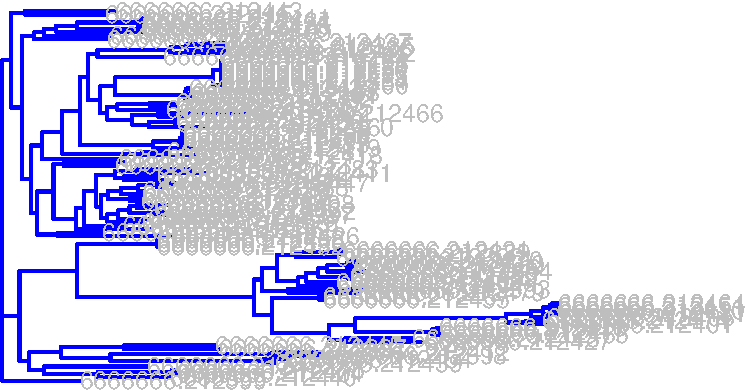
\includegraphics{tesis_files/figure-latex/testingPhylogeny-1} \end{center}
  
  To capture differences on genomes we sort them phylogenetically.
  Phylogenies can be constructed using different paradigms as Parsimony,
  Maximum Likelihood, and Bayesian inference. Short descriptions of the
  main phylogeny methods are included below.
  
  Why is a tree useful \{Book reference\} why trees are useful for?\\
  * Distance methods\\
  * Parsimony * Maximum Likelihood * Mr bayes
  
  General Trees\\
  Actinobacteria Tree, ArchaeaTree, CyanobacteriaTree.
  
  It's easy to create a list. It can be unordered like
  
  To create a sublist, just indent the values a bit (at least four spaces
  or a tab). (Here's one case where indentation is key!)
  
  \begin{enumerate}
  \def\labelenumi{\arabic{enumi}.}
  \tightlist
  \item
    Item 1
  \item
    Item 2
  \item
    Item 3
  
    \begin{itemize}
    \tightlist
    \item
      Item 3a
    \item
      Item 3b
    \end{itemize}
  \end{enumerate}
  
  \subsubsection{Central DB}\label{central-db}
  
  We chose central pathways from (Barona-Gómez, Cruz-Morales, \&
  Noda-García, 2012)\\
  * BBH Best Bidirectional Hits with studied enzymes from Central
  Actinobacterial pathways were selected.
  
  \begin{itemize}
  \item
    By abundance
  \item
    By expansions on genomes
  \end{itemize}
  
  {[}largefiles,\url{https://help.github.com/articles/installing-git-large-file-storage/}{]}
  
  \subsubsection{Natural Products DB}\label{natural-products-db}
  
  Natural products was improved from previous version
  
  \subsection{AntisMASH optional DB}\label{antismash-optional-db}
  
  AntiSMASH is (Weber et al., 2015,Medema et al. (2011))\\
  \#\#\# Archaeas Results Archaea is a kingdom of recent discovery were
  not many natural products has been known. On Actinobacteria, evoMining
  has proved its value to find new kinds of natural products. The clue to
  this discovery was that Actinobacteria has genomic expanssions. Now
  Archaea has genomic expansions, even more has central pathways genomic
  expansions. Are this expansions derived from a genomic duplication?\\
  Has Archaea natural products detected by antismash, and if not, where
  are this NP's or may Archaea doesn't have NP's.
  
  applying EvoMining to Archaea
  
  \subsection{Otras estrategias para los clusters Argon context
  Idea}\label{otras-estrategias-para-los-clusters-argon-context-idea}
  
  Argon When you click the \textbf{Knit} button above a document will be
  generated that includes both content as well as the output of any
  embedded \textbf{R} code chunks within the document. You can embed an
  \textbf{R} code chunk like this (\texttt{cars} is a built-in \textbf{R}
  dataset):
  
  \begin{Shaded}
  \begin{Highlighting}[]
  \KeywordTok{summary}\NormalTok{(cars)}
  \end{Highlighting}
  \end{Shaded}
  
  \begin{verbatim}
       speed           dist       
   Min.   : 4.0   Min.   :  2.00  
   1st Qu.:12.0   1st Qu.: 26.00  
   Median :15.0   Median : 36.00  
   Mean   :15.4   Mean   : 42.98  
   3rd Qu.:19.0   3rd Qu.: 56.00  
   Max.   :25.0   Max.   :120.00  
  \end{verbatim}
  
  \subsection{Inline code}\label{inline-code}
  
  If you'd like to put the results of your analysis directly into your
  discussion, add inline code like this:
  
  \begin{quote}
  The \texttt{cos} of \(2 \pi\) is 1.
  \end{quote}
  
  Another example would be the direct calculation of the standard
  deviation:
  
  \begin{quote}
  The standard deviation of \texttt{speed} in \texttt{cars} is 5.2876444.
  \end{quote}
  
  One last neat feature is the use of the \texttt{ifelse} conditional
  statement which can be used to output text depending on the result of an
  \textbf{R} calculation:
  
  \begin{quote}
  The standard deviation is less than 6.
  \end{quote}
  
  Note the use of \texttt{\textgreater{}} here, which signifies a
  quotation environment that will be indented.
  
  As you see with \texttt{\$2\ \textbackslash{}pi\$} above, mathematics
  can be added by surrounding the mathematical text with dollar signs.
  More examples of this are in {[}Mathematics and Science{]} if you
  uncomment the code in \protect\hyperlink{math}{Math}.
  
  \section{Recomendaciones de Luis}\label{recomendaciones-de-luis}
  
  Para evoMining\\
  Probar distintos métodos de filogenia y después hacer la coloración.\\
  maximum likelihood, Protest phyml\\
  Atracción de ramas largas.\\
  raxml\\
  trim all vs Gblocs (Tony Galvadon)
  
  Comparar dos árboles\\
  Para ver si la evolución de los genes concatenados ha sido simultánea\\
  Robinson and foulds\\
  Joe Felsestein\\
  Phylip
  
  \begin{enumerate}
  \def\labelenumi{\arabic{enumi}.}
  \setcounter{enumi}{1}
  \tightlist
  \item
    dist tree\\
    quarter descomposition\\
    peter gogarten fendou Mao
  \end{enumerate}
  
  Sets de experimentos.\\
  Para el experimento de los streptomyces con ruta centrales el core,
  analizar el problema de dominios múltiples.\\
  Dominios\\
  Nan Song, Dannie durand\\
  Después del blast
  
  Para obtener\\
  Pablo Vinuesa: Get Homologues
  
  Burkhordelias y su toxina (Preguntar a Beto)\\
  Cianobacterias y la ruta de fijación de nitrógeno.
  
  Servidor Viernes a las 12:00
  
  \section{CORASON: Other genome Mining tools
  context-based}\label{corason-other-genome-mining-tools-context-based}
  
  \subsection{CORASoN}\label{corason}
  
  You can also embed plots. For example, here is a way to use the base
  \textbf{R} graphics package to produce a plot using the built-in
  \texttt{pressure} dataset:
  
  \begin{center}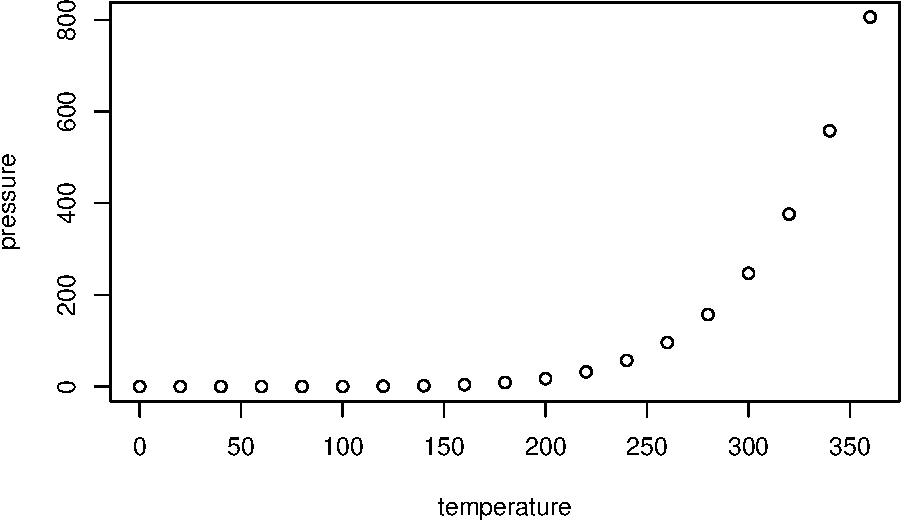
\includegraphics{tesis_files/figure-latex/pressure-1} \end{center}
  
  Note that the \texttt{echo\ =\ FALSE} parameter was added to the code
  chunk to prevent printing of the \textbf{R} code that generated the
  plot. There are plenty of other ways to add chunk options. More
  information is available at \url{http://yihui.name/knitr/options/}.
  
  Another useful chunk option is the setting of \texttt{cache\ =\ TRUE} as
  you see here. If document rendering becomes time consuming due to long
  computations or plots that are expensive to generate you can use knitr
  caching to improve performance. Later in this file, you'll see a way to
  reference plots created in \textbf{R} or external figures.
  
  \section{Loading and exploring data}\label{loading-and-exploring-data}
  
  Included in this template is a file called \texttt{flights.csv}. This
  file includes a subset of the larger dataset of information about all
  flights that departed from Seattle and Portland in 2014. More
  information about this dataset and its \textbf{R} package is available
  at \url{http://github.com/ismayc/pnwflights14}. This subset includes
  only Portland flights and only rows that were complete with no missing
  values. Merges were also done with the \texttt{airports} and
  \texttt{airlines} data sets in the \texttt{pnwflights14} package to get
  more descriptive airport and airline names.
  
  We can load in this data set using the following command:
  
  \begin{Shaded}
  \begin{Highlighting}[]
  \NormalTok{flights <-}\StringTok{ }\KeywordTok{read.csv}\NormalTok{(}\StringTok{"data/flights.csv"}\NormalTok{)}
  \end{Highlighting}
  \end{Shaded}
  
  The data is now stored in the data frame called \texttt{flights} in
  \textbf{R}. To get a better feel for the variables included in this
  dataset we can use a variety of functions. Here we can see the
  dimensions (rows by columns) and also the names of the columns.
  
  \begin{Shaded}
  \begin{Highlighting}[]
  \KeywordTok{dim}\NormalTok{(flights)}
  \end{Highlighting}
  \end{Shaded}
  
  \begin{verbatim}
  [1] 52808    16
  \end{verbatim}
  
  \begin{Shaded}
  \begin{Highlighting}[]
  \KeywordTok{names}\NormalTok{(flights)}
  \end{Highlighting}
  \end{Shaded}
  
  \begin{verbatim}
   [1] "month"        "day"          "dep_time"     "dep_delay"   
   [5] "arr_time"     "arr_delay"    "carrier"      "tailnum"     
   [9] "flight"       "dest"         "air_time"     "distance"    
  [13] "hour"         "minute"       "carrier_name" "dest_name"   
  \end{verbatim}
  
  Another good idea is to take a look at the dataset in table form. With
  this dataset having more than 50,000 rows, we won't explicitly show the
  results of the command here. I recommend you enter the command into the
  Console \textbf{\emph{after}} you have run the \textbf{R} chunks above
  to load the data into \textbf{R}.
  
  \begin{Shaded}
  \begin{Highlighting}[]
  \KeywordTok{View}\NormalTok{(flights)}
  \end{Highlighting}
  \end{Shaded}
  
  While not required, it is highly recommended you use the \texttt{dplyr}
  package to manipulate and summarize your data set as needed. It uses a
  syntax that is easy to understand using chaining operations. Below I've
  created a few examples of using \texttt{dplyr} to get information about
  the Portland flights in 2014. You will also see the use of the
  \texttt{ggplot2} package, which produces beautiful, high-quality
  academic visuals.
  
  We begin by checking to ensure that needed packages are installed and
  then we load them into our current working environment:
  
  \begin{Shaded}
  \begin{Highlighting}[]
  \CommentTok{# List of packages required for this analysis}
  \NormalTok{pkg <-}\StringTok{ }\KeywordTok{c}\NormalTok{(}\StringTok{"dplyr"}\NormalTok{, }\StringTok{"ggplot2"}\NormalTok{, }\StringTok{"knitr"}\NormalTok{, }\StringTok{"devtools"}\NormalTok{)}
  \CommentTok{# Check if packages are not installed and assign the}
  \CommentTok{# names of the packages not installed to the variable new.pkg}
  \NormalTok{new.pkg <-}\StringTok{ }\NormalTok{pkg[!(pkg %in%}\StringTok{ }\KeywordTok{installed.packages}\NormalTok{())]}
  \CommentTok{# If there are any packages in the list that aren't installed,}
  \CommentTok{# install them}
  \NormalTok{if (}\KeywordTok{length}\NormalTok{(new.pkg))}
    \KeywordTok{install.packages}\NormalTok{(new.pkg, }\DataTypeTok{repos =} \StringTok{"http://cran.rstudio.com"}\NormalTok{)}
  \CommentTok{# Load packages}
  \KeywordTok{library}\NormalTok{(dplyr)}
  \KeywordTok{library}\NormalTok{(ggplot2)}
  \KeywordTok{library}\NormalTok{(knitr)}
  \end{Highlighting}
  \end{Shaded}
  
  The example we show here does the following:
  
  \begin{itemize}
  \item
    Selects only the \texttt{carrier\_name} and \texttt{arr\_delay} from
    the \texttt{flights} dataset and then assigns this subset to a new
    variable called \texttt{flights2}.
  \item
    Using \texttt{flights2}, we determine the largest arrival delay for
    each of the carriers.
  \end{itemize}
  
  \begin{Shaded}
  \begin{Highlighting}[]
  \NormalTok{flights2 <-}\StringTok{ }\NormalTok{flights %>%}\StringTok{ }\NormalTok{dplyr::}\KeywordTok{select}\NormalTok{(carrier_name, arr_delay)}
  \NormalTok{max_delays <-}\StringTok{ }\NormalTok{flights2 %>%}\StringTok{ }\KeywordTok{group_by}\NormalTok{(carrier_name) %>%}
  \StringTok{  }\KeywordTok{summarize}\NormalTok{(}\DataTypeTok{max_arr_delay =} \KeywordTok{max}\NormalTok{(arr_delay, }\DataTypeTok{na.rm =} \OtherTok{TRUE}\NormalTok{))}
  \end{Highlighting}
  \end{Shaded}
  
  We next introduce a useful function in the \texttt{knitr} package for
  making nice tables in \emph{R Markdown} called \texttt{kable}. It
  produces the \LaTeX~code required to make the table and is much easier
  to use than manually entering values into a table by copying and pasting
  values into Excel or \LaTeX. This again goes to show how nice
  reproducible documents can be! There is no need to copy-and-paste values
  to create a table. (Note the use of \texttt{results\ =\ "asis"} here
  which will produce the table instead of the code to create the table.
  You'll learn more about the
  \texttt{\textbackslash{}\textbackslash{}label} later.) The
  \texttt{caption.short} argument is used to include a shorter version of
  the title to appear in the List of Tables at the beginning of the
  document.
  
  \begin{Shaded}
  \begin{Highlighting}[]
  \KeywordTok{kable}\NormalTok{(max_delays, }\DataTypeTok{col.names =} \KeywordTok{c}\NormalTok{(}\StringTok{"Airline"}\NormalTok{, }\StringTok{"Max Arrival Delay"}\NormalTok{),}
        \DataTypeTok{caption =} \StringTok{"Maximum Delays by Airline }\CharTok{\textbackslash{}\textbackslash{}}\StringTok{label\{tab:max_delay\}"}\NormalTok{,}
        \DataTypeTok{caption.short =} \StringTok{"Max Delays by Airline"}\NormalTok{)}
  \end{Highlighting}
  \end{Shaded}
  
  \begin{longtable}[c]{@{}lr@{}}
  \caption{Maximum Delays by Airline \label{tab:max_delay}}\tabularnewline
  \toprule
  Airline & Max Arrival Delay\tabularnewline
  \midrule
  \endfirsthead
  \toprule
  Airline & Max Arrival Delay\tabularnewline
  \midrule
  \endhead
  Alaska Airlines Inc. & 338\tabularnewline
  American Airlines Inc. & 1539\tabularnewline
  Delta Air Lines Inc. & 651\tabularnewline
  Frontier Airlines Inc. & 575\tabularnewline
  Hawaiian Airlines Inc. & 407\tabularnewline
  JetBlue Airways & 273\tabularnewline
  SkyWest Airlines Inc. & 421\tabularnewline
  Southwest Airlines Co. & 694\tabularnewline
  United Air Lines Inc. & 472\tabularnewline
  US Airways Inc. & 347\tabularnewline
  Virgin America & 366\tabularnewline
  \bottomrule
  \end{longtable}
  
  We can further look into the properties of the largest value here for
  American Airlines Inc. To do so, we can isolate the row corresponding to
  the arrival delay of 1539 minutes for American in our original
  \texttt{flights} dataset.
  
  \begin{Shaded}
  \begin{Highlighting}[]
  \NormalTok{flights %>%}\StringTok{ }\NormalTok{dplyr::}\KeywordTok{filter}\NormalTok{(arr_delay ==}\StringTok{ }\DecValTok{1539}\NormalTok{, }
                     \NormalTok{carrier_name ==}\StringTok{ "American Airlines Inc."}\NormalTok{) %>%}
  \StringTok{  }\NormalTok{dplyr::}\KeywordTok{select}\NormalTok{(-}\KeywordTok{c}\NormalTok{(month, day, carrier, dest_name, hour, }
              \NormalTok{minute, carrier_name, arr_delay))}
  \end{Highlighting}
  \end{Shaded}
  
  \begin{verbatim}
    dep_time dep_delay arr_time tailnum flight dest air_time distance
  1     1403      1553     1934  N595AA   1568  DFW      182     1616
  \end{verbatim}
  
  We see that the flight occurred on March 3rd and departed a little after
  2 PM on its way to Dallas/Fort Worth. Lastly, we show how we can
  visualize the arrival delay of all departing flights from Portland on
  March 3rd against time of departure.
  
  \begin{Shaded}
  \begin{Highlighting}[]
  \NormalTok{flights %>%}\StringTok{ }\NormalTok{dplyr::}\KeywordTok{filter}\NormalTok{(month ==}\StringTok{ }\DecValTok{3}\NormalTok{, day ==}\StringTok{ }\DecValTok{3}\NormalTok{) %>%}
  \StringTok{  }\KeywordTok{ggplot}\NormalTok{(}\KeywordTok{aes}\NormalTok{(}\DataTypeTok{x =} \NormalTok{dep_time, }\DataTypeTok{y =} \NormalTok{arr_delay)) +}
  \StringTok{  }\KeywordTok{geom_point}\NormalTok{()}
  \end{Highlighting}
  \end{Shaded}
  
  \begin{center}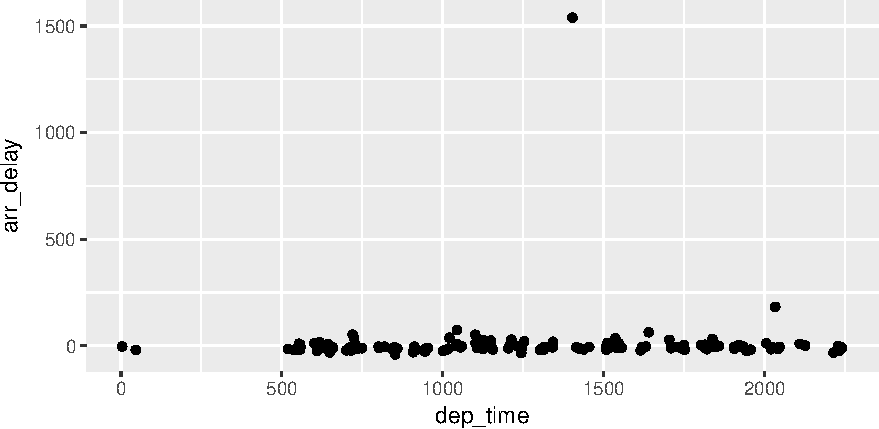
\includegraphics{tesis_files/figure-latex/march3plot-1} \end{center}
  
  \chapter{PriA Family}\label{math-sci}
  
  \begin{itemize}
  \tightlist
  \item
    Julian simulation
  \item
    Who has TrpF
  \end{itemize}
  
  \begin{Shaded}
  \begin{Highlighting}[]
  \CommentTok{# List of packages required for this analysis}
  \NormalTok{pkg <-}\StringTok{ }\KeywordTok{c}\NormalTok{(}\StringTok{"dplyr"}\NormalTok{, }\StringTok{"ggplot2"}\NormalTok{, }\StringTok{"knitr"}\NormalTok{, }\StringTok{"devtools"}\NormalTok{,}\StringTok{" reshape"}\NormalTok{,}\StringTok{"RColorBrewer"}\NormalTok{)}
  \CommentTok{# Check if packages are not installed and assign the}
  \CommentTok{# names of the packages not installed to the variable new.pkg}
  \NormalTok{new.pkg <-}\StringTok{ }\NormalTok{pkg[!(pkg %in%}\StringTok{ }\KeywordTok{installed.packages}\NormalTok{())]}
  \CommentTok{# If there are any packages in the list that aren't installed,}
  \CommentTok{# install them}
  \NormalTok{if (}\KeywordTok{length}\NormalTok{(new.pkg))}
    \KeywordTok{install.packages}\NormalTok{(new.pkg, }\DataTypeTok{repos =} \StringTok{"http://cran.rstudio.com"}\NormalTok{)}
  \end{Highlighting}
  \end{Shaded}
  
  \begin{verbatim}
  Warning: package ' reshape' is not available (for R version 3.3.2)
  \end{verbatim}
  
  \begin{Shaded}
  \begin{Highlighting}[]
  \CommentTok{# Load packages}
  \KeywordTok{library}\NormalTok{(dplyr)}
  \KeywordTok{library}\NormalTok{(plyr)}
  \KeywordTok{library}\NormalTok{(reshape )}
  \KeywordTok{library}\NormalTok{(ggplot2)}
  \KeywordTok{library}\NormalTok{(knitr)}
  \KeywordTok{library}\NormalTok{(RColorBrewer)}
  \NormalTok{hm.palette <-}\StringTok{ }\KeywordTok{colorRampPalette}\NormalTok{(}\KeywordTok{rev}\NormalTok{(}\KeywordTok{brewer.pal}\NormalTok{(}\DecValTok{11}\NormalTok{, }\StringTok{'Spectral'}\NormalTok{)), }\DataTypeTok{space=}\StringTok{'Lab'}\NormalTok{)  }
  \end{Highlighting}
  \end{Shaded}
  
  \hypertarget{math}{\section{Math}\label{math}}
  
  Docking simulation were calculated for Streptomyces enzymes
  
  Procedures can be found at
  \href{https://github.com/tripplab/Docking/wiki}{Docking Protocols}
  
  1.Phylogenetic Tree 39 Streptomyces sequences, as outgroup E coli,
  Arthrobacter Aurescens, Salmonella enterica and Acidimicrobium
  ferrooxidans PriA's were included.
  
  CORASON PriA All streptomyces have a partially conserved PriA cluster.
  CT34 has a secondary copy whose Best hit on NCBI is Lentzea's PriA with
  50\% identity 98\% coverage
  
  TrpF1 TrpF1 queries gave hits with TrpC enzyme present on every
  Streptomyces, additionally S rimosus, S coelicolor, S venezuelae and S.
  NRRL S-1813 had an extra copy. S rimosus TrpC vicinity has PKS and
  siderophore genes.
  
  TrpF2 Conserved cluster with NRPS sequences flanking TrpF2
  
  TrpF3 Non conserved cluster
  
  TrpF4 purpeofuscus and S bikiniensis 2. Heatmap Additionally to the
  sequences selected by phylogeny, Jonesia denitrificans and Streptomyces
  sp Mg1 TrpF sequences were added as control .
  
  \begin{Shaded}
  \begin{Highlighting}[]
  \KeywordTok{library}\NormalTok{(genstats)}
  \KeywordTok{library}\NormalTok{(devtools)}
  \KeywordTok{library}\NormalTok{(Biobase)}
  \end{Highlighting}
  \end{Shaded}
  
  \begin{verbatim}
  Loading required package: BiocGenerics
  \end{verbatim}
  
  \begin{verbatim}
  Loading required package: parallel
  \end{verbatim}
  
  \begin{verbatim}
  
  Attaching package: 'BiocGenerics'
  \end{verbatim}
  
  \begin{verbatim}
  The following objects are masked from 'package:parallel':
  
      clusterApply, clusterApplyLB, clusterCall, clusterEvalQ,
      clusterExport, clusterMap, parApply, parCapply, parLapply,
      parLapplyLB, parRapply, parSapply, parSapplyLB
  \end{verbatim}
  
  \begin{verbatim}
  The following objects are masked from 'package:dplyr':
  
      combine, intersect, setdiff, union
  \end{verbatim}
  
  \begin{verbatim}
  The following objects are masked from 'package:stats':
  
      IQR, mad, xtabs
  \end{verbatim}
  
  \begin{verbatim}
  The following objects are masked from 'package:base':
  
      anyDuplicated, append, as.data.frame, cbind, colnames,
      do.call, duplicated, eval, evalq, Filter, Find, get, grep,
      grepl, intersect, is.unsorted, lapply, lengths, Map, mapply,
      match, mget, order, paste, pmax, pmax.int, pmin, pmin.int,
      Position, rank, rbind, Reduce, rownames, sapply, setdiff,
      sort, table, tapply, union, unique, unsplit, which, which.max,
      which.min
  \end{verbatim}
  
  \begin{verbatim}
  Welcome to Bioconductor
  
      Vignettes contain introductory material; view with
      'browseVignettes()'. To cite Bioconductor, see
      'citation("Biobase")', and for packages 'citation("pkgname")'.
  \end{verbatim}
  
  \begin{Shaded}
  \begin{Highlighting}[]
  \KeywordTok{sessionInfo}\NormalTok{()}
  \end{Highlighting}
  \end{Shaded}
  
  \begin{verbatim}
  R version 3.3.2 (2016-10-31)
  Platform: x86_64-pc-linux-gnu (64-bit)
  Running under: Ubuntu 14.04.5 LTS
  
  locale:
   [1] LC_CTYPE=en_US.UTF-8       LC_NUMERIC=C              
   [3] LC_TIME=es_MX.UTF-8        LC_COLLATE=en_US.UTF-8    
   [5] LC_MONETARY=es_MX.UTF-8    LC_MESSAGES=en_US.UTF-8   
   [7] LC_PAPER=es_MX.UTF-8       LC_NAME=C                 
   [9] LC_ADDRESS=C               LC_TELEPHONE=C            
  [11] LC_MEASUREMENT=es_MX.UTF-8 LC_IDENTIFICATION=C       
  
  attached base packages:
  [1] parallel  stats     graphics  grDevices utils     datasets  methods  
  [8] base     
  
  other attached packages:
   [1] Biobase_2.34.0      BiocGenerics_0.20.0 genstats_0.1.02    
   [4] RColorBrewer_1.1-2  reshape_0.8.6       plyr_1.8.4         
   [7] knitr_1.15.1        ggplot2_2.2.1       dplyr_0.5.0        
  [10] ape_4.0             reedtemplates_0.1   devtools_1.12.0    
  
  loaded via a namespace (and not attached):
   [1] Rcpp_0.12.9      magrittr_1.5     munsell_0.4.3    colorspace_1.3-2
   [5] lattice_0.20-34  R6_2.2.0         highr_0.6        stringr_1.1.0   
   [9] tools_3.3.2      grid_3.3.2       nlme_3.1-129     gtable_0.2.0    
  [13] DBI_0.5-1        withr_1.0.2      htmltools_0.3.5  lazyeval_0.2.0  
  [17] yaml_2.1.14      rprojroot_1.2    digest_0.6.12    assertthat_0.1  
  [21] tibble_1.2       memoise_1.0.0    evaluate_0.10    rmarkdown_1.3   
  [25] labeling_0.3     stringi_1.1.2    scales_0.4.1     backports_1.0.5 
  \end{verbatim}
  
  \begin{Shaded}
  \begin{Highlighting}[]
  \CommentTok{#vignette(package="genstats")}
  \CommentTok{#vignette("01_06_three-tables")}
  
  \CommentTok{# phenoData:}
  \NormalTok{tmp <-}\StringTok{ }\KeywordTok{read.csv}\NormalTok{(}\StringTok{"chapter2/ProteinData"}\NormalTok{, }\DataTypeTok{row.names =} \DecValTok{1}\NormalTok{,}\DataTypeTok{header=}\OtherTok{TRUE}\NormalTok{,}\DataTypeTok{sep=}\StringTok{"}\CharTok{\textbackslash{}t}\StringTok{"}\NormalTok{)}
  \NormalTok{pdata <-}\StringTok{ }\KeywordTok{AnnotatedDataFrame}\NormalTok{(tmp)}
  
    \CommentTok{# featureData:}
  \NormalTok{tmp <-}\StringTok{ }\KeywordTok{read.csv}\NormalTok{(}\StringTok{"chapter2/Substrate.data"}\NormalTok{, }\DataTypeTok{row.names =} \DecValTok{1}\NormalTok{,}\DataTypeTok{sep=}\StringTok{"}\CharTok{\textbackslash{}t}\StringTok{"}\NormalTok{)}
  \NormalTok{fdata <-}\StringTok{ }\KeywordTok{AnnotatedDataFrame}\NormalTok{(tmp)}
  
  \CommentTok{# expression data:}
  \NormalTok{tmp <-}\StringTok{ }\KeywordTok{read.table}\NormalTok{(}\StringTok{"chapter2/EnsymeVsSubstrate.data"}\NormalTok{,}\DataTypeTok{row.names =} \DecValTok{1}\NormalTok{,}\DataTypeTok{header=}\OtherTok{TRUE}\NormalTok{,}\DataTypeTok{sep=}\StringTok{"}\CharTok{\textbackslash{}t}\StringTok{"}\NormalTok{)}
  \NormalTok{m <-}\StringTok{ }\KeywordTok{as.matrix}\NormalTok{(tmp)}
  \CommentTok{#dim(m)}
  \CommentTok{#class(m)}
  \CommentTok{#colnames(m)}
  \CommentTok{#rownames(m)}
  \NormalTok{## Names should not start on numbers never}
  \NormalTok{## create ExpressionSet object:}
  \NormalTok{eset <-}\StringTok{ }\KeywordTok{new}\NormalTok{(}\StringTok{"ExpressionSet"}\NormalTok{, }\DataTypeTok{exprs =} \NormalTok{m, }\DataTypeTok{phenoData =} \NormalTok{pdata, }\DataTypeTok{featureData =} \NormalTok{fdata)}
  
  \CommentTok{#pData(eset)}
  \CommentTok{#fData(eset)}
  \CommentTok{#pData(eset)}
  \CommentTok{#fData(eset)}
  \end{Highlighting}
  \end{Shaded}
  
  \begin{Shaded}
  \begin{Highlighting}[]
  \NormalTok{docking <-}\StringTok{ }\KeywordTok{read.csv}\NormalTok{(}\StringTok{"chapter2/Heat.data"}\NormalTok{, }\DataTypeTok{header=}\OtherTok{TRUE}\NormalTok{, }\DataTypeTok{sep=}\StringTok{"}\CharTok{\textbackslash{}t}\StringTok{"}\NormalTok{)}
  \NormalTok{docking.m <-}\StringTok{ }\KeywordTok{melt}\NormalTok{(docking,}\DataTypeTok{id =} \StringTok{"Enzima"}\NormalTok{)}
  \CommentTok{#docking.m<- ddply(docking.m, .(docking.m$variable), transform, rescale=scale(value))  ## rescale escala toda la matriz, scale por columnas}
  \NormalTok{## NEcesito escalar!!!}
  
  
  \KeywordTok{ggplot}\NormalTok{(docking.m, }\KeywordTok{aes}\NormalTok{(}\DataTypeTok{x=}\NormalTok{docking.m$variable, }\DataTypeTok{y=}\NormalTok{docking.m$Enzima)) +}\StringTok{ }\KeywordTok{labs}\NormalTok{(}\DataTypeTok{x =} \StringTok{"Substrates"}\NormalTok{, }\DataTypeTok{y =} \StringTok{"Enzymes"}\NormalTok{,}\DataTypeTok{text =} \KeywordTok{element_text}\NormalTok{(}\DataTypeTok{size=}\DecValTok{12}\NormalTok{))+}\StringTok{ }\KeywordTok{geom_raster}\NormalTok{(}\KeywordTok{aes}\NormalTok{(}\DataTypeTok{fill=}\NormalTok{docking.m$value))+}\KeywordTok{theme_bw}\NormalTok{()+}\KeywordTok{theme}\NormalTok{(}\DataTypeTok{plot.title =} \KeywordTok{element_text}\NormalTok{(}\DataTypeTok{size =} \DecValTok{14}\NormalTok{, }\DataTypeTok{face =} \StringTok{"bold"}\NormalTok{), }\DataTypeTok{text =} \KeywordTok{element_text}\NormalTok{(}\DataTypeTok{size =} \DecValTok{12}\NormalTok{), }\DataTypeTok{axis.title =} \KeywordTok{element_text}\NormalTok{(}\DataTypeTok{face=}\StringTok{"bold"}\NormalTok{), }\DataTypeTok{axis.text.x=}\KeywordTok{element_text}\NormalTok{(}\DataTypeTok{angle =} \DecValTok{90}\NormalTok{,}\DataTypeTok{size =} \DecValTok{6}\NormalTok{))}
  \end{Highlighting}
  \end{Shaded}
  
  \begin{center}\includegraphics{tesis_files/figure-latex/load_data_docking-1} \end{center}
  
  \begin{Shaded}
  \begin{Highlighting}[]
  \CommentTok{#+scale_fill_gradient(low = "white", high = "black",na.value = "orange")}
  \CommentTok{#+ scale_fill_gradientn(colours = hm.palette(100),na.value = "gray")}
  
  
  \CommentTok{#ggplot(docking.m, aes(x=docking.m$variable, y=docking.m$Enzima))+ geom_raster(aes(fill=docking.m$value)) +}
  \CommentTok{#  theme(text = element_text(size=8), axis.text.x = element_text(angle = 90, hjust = 1, vjust = 0.5)) +}
  \CommentTok{#  coord_equal()+scale_fill_gradient(low = "white", high = "black",na.value = "orange")}
  \end{Highlighting}
  \end{Shaded}
  
  We next introduce a useful function in the \texttt{knitr} package for
  making nice tables in \emph{R Markdown} called \texttt{kable}. It
  produces the \LaTeX~code required to make the table and is much easier
  to use than manually entering values into a table by copying and pasting
  values into Excel or \LaTeX. This again goes to show how nice
  reproducible documents can be! There is no need to copy-and-paste values
  to create a table. (Note the use of \texttt{results\ =\ "asis"} here
  which will produce the table instead of the code to create the table.
  You'll learn more about the
  \texttt{\textbackslash{}\textbackslash{}label} later.) The
  \texttt{caption.short} argument is used to include a shorter version of
  the title to appear in the List of Tables at the beginning of the
  document.
  
  \begin{Shaded}
  \begin{Highlighting}[]
  \KeywordTok{kable}\NormalTok{(docking,  }\DataTypeTok{caption =} \StringTok{"Enzymes docking }\CharTok{\textbackslash{}\textbackslash{}}\StringTok{label\{tab:docking\}"}\NormalTok{,}\DataTypeTok{caption.short =} \StringTok{"Enzymes docking "}\NormalTok{)}
  \end{Highlighting}
  \end{Shaded}
  
  \begin{longtable}[c]{@{}lllllllllllllllllllll@{}}
  \caption{Enzymes docking \label{tab:docking}}\tabularnewline
  \toprule
  Enzima & dte6\_open & dte13\_open & dte6\_closed & dte13\_closed &
  C04376 & C03838 & C04640 & CompoundV & C05923 & C05922 & C01268 & PraP &
  C04302 & C00144 & C00044 & C01253 & C01201 & C04896 & X17146 &
  X16827\tabularnewline
  \midrule
  \endfirsthead
  \toprule
  Enzima & dte6\_open & dte13\_open & dte6\_closed & dte13\_closed &
  C04376 & C03838 & C04640 & CompoundV & C05923 & C05922 & C01268 & PraP &
  C04302 & C00144 & C00044 & C01253 & C01201 & C04896 & X17146 &
  X16827\tabularnewline
  \midrule
  \endhead
  5AHE\_Senterica & -9.1 & -5.4 & -6.4 & -5.2 & -8 & -7.3 & -7.4 & -8.8 &
  -10.7 & -10.2 & -8.7 & -8.7 & -9.6 & -9.9 & -10.9 & -7.8 & -9.1 & -10.3
  & -9 & -8.4\tabularnewline
  Coli\_K12 & -9.7 & -9.7 & -9.2 & -6.1 & -7.2 & -6.6 & -6.8 & -8.6 & -9.5
  & -9.1 & -8.6 & -8.2 & -9 & -8.6 & -10.2 & -9.9 & -10.2 & -9.9 & -8.2 &
  -7.9\tabularnewline
  Acidimicrobium & -5.7 & -5.8 & -6 & -5.7 & -6.7 & -6.2 & -5.8 & -7.6 &
  -9.2 & -8.8 & -7.8 & -7.4 & -8.3 & -8.4 & -9.3 & -6.7 & -4.5 & -9.1 &
  -8.3 & -8.1\tabularnewline
  JOAQ01 & -7.4 & -7.3 & -7.5 & -7.1 & -6.5 & -6.2 & -6.5 & -7.7 & -9.4 &
  -9.3 & -7.9 & -7.2 & -8.3 & -8.6 & -8.9 & -9 & -7.1 & -8.9 & -7.8 &
  -7.7\tabularnewline
  2VEP & -7.5 & -7.5 & -7.9 & -7 & -7 & -6.2 & -6.5 & -7.8 & -8.8 & -9.2 &
  -7.8 & -7.9 & -8 & -8.9 & -10.3 & -9.2 & -9.3 & -8.4 & -8.1 &
  -8.2\tabularnewline
  2X30 & -8.1 & -7.4 & -7.6 & -6.9 & -6.7 & -6.8 & -7.1 & -7.9 & -9.1 & -9
  & -8.3 & -8.6 & -8.5 & -9 & -10.6 & -10 & -10.3 & -10.2 & -8.1 &
  -7.9\tabularnewline
  1VZW & na & na & na & na & na & na & na & na & na & na & na & na & na &
  na & na & na & na & na & na & na\tabularnewline
  JOFS01 & -7.2 & -6.7 & -6.8 & -6.5 & -6.2 & -6.6 & -5.9 & -7.8 & -8.5 &
  -7.8 & -7.8 & -7.2 & -8.2 & -8 & -9.6 & -8.2 & -8 & -9.4 & -7.7 &
  -7.5\tabularnewline
  BAVY01 & -7.4 & -7.2 & -7 & -6.5 & -7.3 & -6.4 & -7 & -7.5 & -9.6 & -8.5
  & -7.9 & -7.6 & -8.4 & -8.7 & -9.8 & -8.3 & -7.9 & -8.6 & -7.7 &
  -7.6\tabularnewline
  JOCU01 & -7.1 & -7.6 & -7.2 & -7.3 & -7.2 & -6.8 & -6.9 & -8.1 & -8.2 &
  -7.2 & -8.2 & -7.2 & -8.4 & -8.3 & -8.5 & -7.9 & -7.8 & -6 & -7.5 &
  -7.3\tabularnewline
  ABYA01 & -9.2 & -8.7 & -6.7 & -6.7 & -7.4 & -7.7 & -7.2 & -7.5 & -9.8 &
  -8.9 & -8.2 & -7.8 & -8.8 & -8.7 & -10.1 & -9.1 & -9 & -9.5 & -8 &
  -7.5\tabularnewline
  JNXI01 & -6.6 & -7.3 & -7 & -7.1 & -7.1 & -7.1 & -6.8 & -8 & -9.2 & -8.7
  & -7.8 & -7.6 & -8.3 & -8.4 & -9.1 & -5.8 & -5.3 & -8.5 & -7.3 &
  -7.4\tabularnewline
  ABYC01 & -6.3 & -7.1 & -7.4 & -6.8 & -7.7 & -6.9 & -6.6 & -8 & -9.6 &
  -8.9 & -8.6 & -7.9 & -8.6 & -8.4 & -9.1 & -7.4 & -7.2 & -8.8 & -8.1 &
  -7.8\tabularnewline
  JOFG01 & -7.3 & -8.8 & -7.5 & -6.7 & -7 & -6.5 & -6.5 & -8.7 & -10 &
  -9.7 & -8.8 & -7.7 & -8.2 & -8.6 & -10.5 & -8.1 & -9.2 & -8.9 & -7.6 &
  -7.6\tabularnewline
  JNZV01 & -8.9 & -6.6 & -6.7 & -6.8 & -7.2 & -7.2 & -6.2 & -7.7 & -9.6 &
  -9.5 & -8.4 & -7.4 & -8.5 & -8.2 & -9.7 & -8.5 & -8.4 & -9.3 & -7.4 &
  -7.7\tabularnewline
  AJUO01 & -6.1 & -6.8 & -6.9 & -6.5 & -6.7 & -6.3 & -6.7 & -7.5 & -9.6 &
  -9.6 & -8.6 & -7.8 & -8.7 & -8.7 & -9.9 & -6.2 & -5.1 & -9.2 & -7.8 &
  -7.7\tabularnewline
  JNXH01 & -9 & -6.9 & -7.1 & -6.8 & -6.3 & -7.2 & -6.6 & -8.1 & -9.8 &
  -9.3 & -7.7 & -8 & -8.7 & -8.8 & -10.5 & -7.6 & -9.1 & -10.5 & -7.1 &
  -7.4\tabularnewline
  JOFC01 & -6.6 & -8.2 & -7.1 & -6.4 & -7.1 & -7.4 & -7.1 & -7.4 & -9.4 &
  -8.5 & -8.6 & -7.5 & -8.8 & -8.4 & -9.6 & -8.8 & -8.8 & -8.7 & -7.7 &
  -7.5\tabularnewline
  JNWL01 & -7.4 & -6.7 & -7.4 & -7.3 & -7.7 & -6.5 & -6.8 & -8.5 & -9.9 &
  -9.8 & -8.3 & -7.8 & -8.2 & -8.4 & -10.5 & -7.1 & -6.3 & -8.3 & -8.1 &
  -7.9\tabularnewline
  AJSZ01 & -6.9 & -7.5 & -7.9 & -7.8 & -7.5 & -7.3 & -7.7 & -8.1 & -10 &
  -9.7 & -8.7 & -7.8 & -8.8 & -8.8 & -10.6 & -7.8 & -8.7 & -9.2 & -7.9 &
  -7.8\tabularnewline
  10712 & -8.3 & -7.6 & -7.5 & -6.8 & -6.4 & -7 & -6.2 & -8.2 & -9.6 & -9
  & -7.9 & -7.4 & -8.3 & -8.6 & -10 & -8.2 & -8.2 & -8.1 & -7.6 &
  -7.4\tabularnewline
  JSFP01 & -7.8 & -7.2 & -7.6 & -7.3 & -6.2 & -6.5 & -6.9 & -8 & -8.8 &
  -8.6 & -7.7 & -7.1 & -7.7 & -7.9 & -7.2 & -7.1 & -6.7 & -7.1 & -7.7 &
  -7.7\tabularnewline
  JJNO01 & -7.4 & -6.8 & -7.1 & -7.2 & -7.2 & -7.4 & -7.8 & -8.6 & -9.7 &
  -9.3 & -8.8 & -7.7 & -8.9 & -8.7 & -10.2 & -6.8 & -8.2 & -9 & -7.5 &
  -7.8\tabularnewline
  JQJU01 & -7.6 & -7.1 & -7.5 & -7.4 & -6.2 & -6.5 & -6.9 & -8 & -8.9 &
  -8.7 & -7.7 & -7.4 & -7.7 & -7.8 & -6.5 & -7 & -6.3 & -7.7 & -7.7 &
  -7.7\tabularnewline
  JOHB01 & -7.5 & -6.7 & -6.8 & -6.6 & -6.8 & -7 & -6.7 & -7.9 & -9.9 &
  -9.7 & -8.3 & -7.7 & -8.5 & -8.6 & -10 & -7.6 & -7.5 & -8.6 & -7.3 &
  -7.5\tabularnewline
  JOBF01 & -6.3 & -6.8 & -7 & -6.3 & -6.9 & -6.9 & -6.6 & -7.8 & -9.3 &
  -7.4 & -8.5 & -7.3 & -8 & -8.7 & -8.5 & -7.4 & -6.3 & -6 & -7.9 &
  -7.5\tabularnewline
  JNAD01 & -7.3 & -7 & -6.8 & -6.6 & -6.5 & -7.3 & -6.6 & -8.6 & -9.1 &
  -8.7 & -8.9 & -7.7 & -8.9 & -9 & -8.7 & -6 & -6.3 & -7.9 & -8.2 &
  -7.8\tabularnewline
  ARLC01 & -7.5 & -7 & -6.9 & -6.6 & -6.6 & -6.7 & -6.9 & -7.7 & -8.4 &
  -8.2 & -8.2 & -7.5 & -8.1 & -7.7 & -8.2 & -6.7 & -7.1 & -7.7 & -7.6 &
  -7.4\tabularnewline
  JODL01 & -8 & -7.3 & -6.9 & -6.6 & -7.2 & -6.7 & -6.1 & -7.6 & -9.2 &
  -9.1 & -7.8 & -7.4 & -8.2 & -8.5 & -9.6 & -9.2 & -9.2 & -8.6 & -7.7 &
  -7.5\tabularnewline
  ADGD01 & -6.4 & -7.7 & -7.4 & -7.2 & -7.6 & -7.5 & -7.2 & -8.5 & -10.1 &
  -10 & -8.7 & -7.9 & -8.8 & -9.1 & -10.2 & -6.9 & -8.1 & -8.5 & -7.7 &
  -7.7\tabularnewline
  ARTP01 & -9.6 & -10.9 & -8.9 & -7.1 & -6 & -6.2 & -6.7 & -8.1 & -9.1 &
  -8.8 & -8.3 & -7.9 & -8.9 & -9.3 & -9.4 & -9.8 & -10 & -8.9 & -8.2 &
  -8\tabularnewline
  AEJC01 & -6.6 & -6.6 & -7.3 & -6.9 & -6.5 & -6.3 & -6.5 & -8.1 & -8.6 &
  -9.1 & -8 & -7.9 & -8 & -8.4 & -8.5 & -7.2 & -8.4 & -8.2 & -7.9 &
  -7.6\tabularnewline
  ABJJ02 & -5.9 & -8.2 & -7.1 & -6.6 & -6.8 & -7 & -7.6 & -7.9 & -8.4 &
  -8.3 & -8.2 & -8.1 & -8.4 & -8.7 & -7.7 & -8.2 & -8.2 & -6.7 & -8 &
  -7.5\tabularnewline
  4U28 & na & na & na & na & na & na & na & na & na & na & na & na & na &
  na & na & na & na & na & na & na\tabularnewline
  4TX9 & na & na & na & na & na & na & na & na & na & na & na & na & na &
  na & na & na & na & na & na & na\tabularnewline
  JOBU01 & -8 & -7.1 & -6.7 & -6.9 & -6.6 & -6.8 & -6.7 & -8.2 & -9.5 &
  -9.1 & -8.6 & -8 & -8.4 & -8.7 & -9.1 & -9.5 & -9.3 & -8.1 & -8.1 &
  -7.6\tabularnewline
  JNZG01 & -7.8 & -7.2 & -7.6 & -7.2 & -7.4 & -6.9 & -7.4 & -8.5 & -9.4 &
  -9.4 & -8.6 & -7.6 & -8.4 & -8.6 & -9.1 & -10 & -10.1 & -9 & -7.8 &
  -8.2\tabularnewline
  JNZY01 & -6.4 & -7 & -7.1 & -6.7 & -7.7 & -6.3 & -6.2 & -8.1 & -8.5 &
  -9.2 & -8.3 & -7.6 & -9 & -8.5 & -9.7 & -9.5 & -9.9 & -9.2 & -7.4 &
  -7.5\tabularnewline
  JNZH01 & -7.5 & -6.9 & -6.8 & -6.8 & -6.5 & -6.6 & -6.5 & -8.3 & -8 &
  -8.1 & -7.6 & -7.4 & -8.7 & -8.1 & -8.1 & -8.5 & -8 & -7.6 & -7.7 &
  -7.4\tabularnewline
  ACEW01 & -7.4 & -6.9 & -7.3 & -6.8 & -7.3 & -6.6 & -7.5 & -8 & -9.8 &
  -9.3 & -8.7 & -7.6 & -8.5 & -8.4 & -10.6 & -9.1 & -8.9 & -8.5 & -8.1 &
  -8\tabularnewline
  ATCJ01 & -6.5 & -6.9 & -7.2 & -7.1 & -6.5 & -6.9 & -6.4 & -7.3 & -7.8 &
  -7.7 & -8.3 & -7.5 & -7.9 & -8.4 & -9.5 & -7.6 & -5.2 & -7.5 & -7.6 &
  -7.7\tabularnewline
  4X9S & na & na & na & na & na & na & na & na & na & na & na & na & na &
  na & na & na & na & na & na & na\tabularnewline
  4W9T & na & na & na & na & na & na & na & na & na & na & na & na & na &
  na & na & na & na & na & na & na\tabularnewline
  AWQW01 & -6.2 & -6.8 & -7.4 & -6.5 & -7.8 & -6.8 & -6.7 & -9.5 & -9.6 &
  -9.4 & -8.7 & -8.2 & -8.6 & -9.1 & -9.9 & -5.4 & -5.5 & -9.2 & -8 &
  -7.5\tabularnewline
  JOFK01 & -7.6 & -6.7 & -7.1 & -7.2 & -7.1 & -6.5 & -6.6 & -7.8 & -8.6 &
  -10 & -8.6 & -7.5 & -8.3 & -8.5 & -8.8 & -5.3 & -5.2 & -5.8 & -7.7 &
  -7.4\tabularnewline
  JODS01 & -6.8 & -7.3 & -6.9 & -6.7 & -8 & -7.9 & -7.7 & -8.5 & -9.5 &
  -9.8 & -8.1 & -7.8 & -8.7 & -9.7 & -10 & -5.3 & -6.2 & -8.2 & -7.6 &
  -7.4\tabularnewline
  TC1 & -8.2 & -8.5 & -8.1 & -7.9 & -5.7 & -5.5 & -5.9 & -7 & -7.5 & -7.2
  & -7.1 & -6.7 & -7.1 & -7.4 & -8.4 & -7.2 & -7.3 & -7.4 & -7 &
  -6.7\tabularnewline
  4WD0\_TC1 & na & na & na & na & na & na & na & na & na & na & na & na &
  na & na & na & na & na & na & na & na\tabularnewline
  Auro 4X2R & -9.9 & -9.1 & -9.8 & -8.1 & -7.4 & -7.1 & -7.4 & -7.8 & -9.2
  & -9.8 & -8.3 & -7.8 & -9.3 & -9 & -9.9 & -9 & -8.6 & -9.2 & -8.5 &
  -8.2\tabularnewline
  Acardi\_b2 & -10.6 & -9.3 & -9.3 & -7.2 & -7.2 & -6.8 & -7.3 & -7.5 &
  -9.5 & -9.8 & -8 & -7.8 & -9.3 & -8.9 & -10.3 & -9.6 & -9.4 & -9.4 &
  -8.1 & -8\tabularnewline
  JNZF01 & -6.9 & -6.8 & -7.5 & -7.1 & -7.8 & -7.3 & -7.2 & -8.3 & -9.2 &
  -8.3 & -8.9 & -8.4 & -8.9 & -9.3 & -9.4 & -5.3 & -5.2 & -7.1 & -8.5 &
  -8.6\tabularnewline
  2Y88 & -10 & -7.8 & -8.9 & -5.4 & -8.6 & -7.3 & -7.8 & -9.5 & -10.9 &
  -10.3 & -9.5 & -9 & -9.8 & -9.8 & -11.3 & -10.1 & -10.2 & -11.3 & -9.5 &
  -8.8\tabularnewline
  2Y89 & -8.7 & -8.6 & -9.6 & -9.4 & -6.4 & -5.9 & -5.6 & -7.1 & -7 & -7.5
  & -7.3 & -6.8 & -7.4 & -8.4 & -7.5 & -8.1 & -8.6 & -7.5 & -7.7 &
  -7.3\tabularnewline
  2Y85 & -8.2 & -7.9 & -9.2 & -7.4 & -7.6 & -7.5 & -7.6 & -8.4 & -9.7 &
  -9.5 & -9.3 & -7.8 & -8.6 & -8.6 & -10.2 & -9.8 & -9.9 & -10.1 & -7.3 &
  -7.4\tabularnewline
  3ZS4 & -10 & -10.5 & -11.4 & -6.4 & -8.2 & -7.2 & -7 & -9.6 & -10.2 &
  -10.2 & -9.9 & -8.5 & -9.3 & -9.6 & -10.9 & -10 & -10.7 & -9.9 & -8.8 &
  -8.9\tabularnewline
  diphtheriae & -9.2 & -7.8 & -10.9 & -7.2 & -7.5 & -7.6 & -7.7 & -8.9 &
  -9 & -9.8 & -9 & -8.3 & -8.8 & -9.2 & -10.1 & -9.5 & -9.9 & -9.2 & -8 &
  -7.9\tabularnewline
  jeikeium & -7.5 & -6.9 & -7.2 & -6.5 & -8.4 & -8 & -8.5 & -8.7 & -9.5 &
  -9.6 & -9.4 & -8.8 & -9 & -9.5 & -9.3 & -8.1 & -9.3 & -8.5 & -7.9 &
  -7.7\tabularnewline
  JSFP01\_2 & -7.4 & -8 & -7.6 & -6.4 & -5.2 & -5.4 & -5.2 & -6.1 & -6.8 &
  -6.4 & -5.7 & -6.4 & -6.3 & -6.3 & -7.1 & -7.4 & -7.1 & -6.4 & -7.1 &
  -6.6\tabularnewline
  TrpF Jonesia 4WUI & -8.3 & -8.8 & -8.2 & -6.8 & -6.2 & -6.1 & -6 & -6.8
  & -7.4 & -7.6 & -7.5 & -6.9 & -7.6 & -7.5 & -7.7 & -7.5 & -7.6 & -7.2 &
  -7.3 & -7.2\tabularnewline
  trachomatis & -8.2 & -8 & -7.4 & -7.2 & -6.1 & -5.5 & -5.4 & -6.5 & -7.1
  & -7.1 & -7 & -6.2 & -6.8 & -6.8 & -6.9 & -7.2 & -7.4 & -6.5 & -6.7 &
  -6.6\tabularnewline
  mg1 & -7.2 & -8.8 & -8.2 & -7.3 & -6.2 & -5.7 & -5.7 & -6.9 & -6.6 &
  -6.7 & -7.3 & -6.7 & -7.6 & -6.9 & -7.5 & -7.1 & -7.1 & -6.9 & -6.7 &
  -6.5\tabularnewline
  Aodo\_b12 & -8.5 & -8.6 & -8.8 & -7.3 & -7.1 & -7.1 & -7.1 & -7.5 & -9.7
  & -9.4 & -7.8 & -7.6 & -9.6 & -8.8 & -10.1 & -8.4 & -8.9 & -9.4 & -8 &
  -8.1\tabularnewline
  \bottomrule
  \end{longtable}
  
  We can further look into the properties of the largest value here for
  American Airlines Inc. To do so, we can isolate the row corresponding to
  the arrival delay of 1539 minutes for American in our original
  \texttt{flights} dataset.
  
  \begin{Shaded}
  \begin{Highlighting}[]
  \CommentTok{#flights %>% dplyr::filter(arr_delay == 1539, carrier_name == "American Airlines Inc.") %>%}
    \CommentTok{#dplyr::select(-c(month, day, carrier, dest_name, hour, minute, carrier_name, arr_delay))}
  \end{Highlighting}
  \end{Shaded}
  
  We see that the flight occurred on March 3rd and departed a little after
  2 PM on its way to Dallas/Fort Worth. Lastly, we show how we can
  visualize the arrival delay of all departing flights from Portland on
  March 3rd against time of departure.
  
  \begin{Shaded}
  \begin{Highlighting}[]
  \CommentTok{#flights %>% dplyr::filter(month == 3, day == 3) %>%}
  \CommentTok{#  ggplot(aes(x = dep_time, y = arr_delay)) +geom_point()}
  \end{Highlighting}
  \end{Shaded}
  
  Genome size vs Total antismash cluster coloured by order
  
  \begin{figure}[h!tbp]
  \centering
  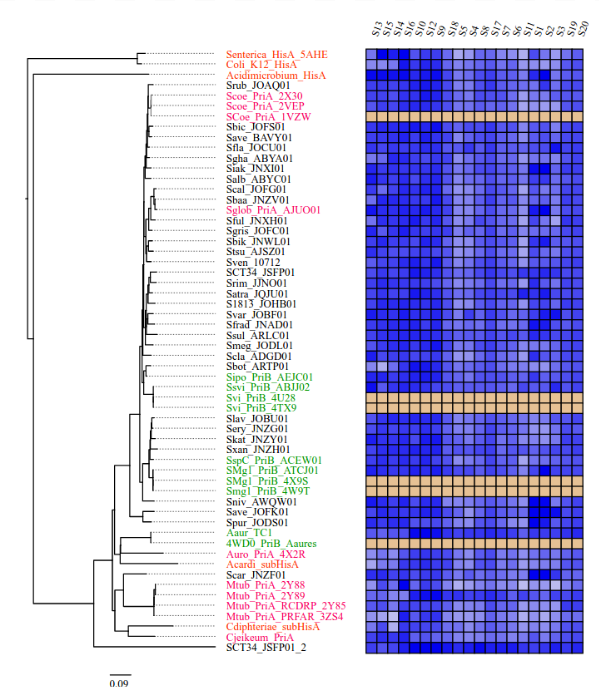
\includegraphics[angle = 0,scale = 0.6]{chapter2/PriAHeatPot.png}
  \caption[Heat Plot PriA Streptomyces vs other subtrates]{\normalsize{Heat Plot PriA Streptomyces vs other subtrates}}
  \label{fig:PriADocking}
  \end{figure}
  
  Docker simulation were calculated for Streptomyces enzymes\\
  Genome size vs Total antismash cluster coloured by order
  
  \begin{figure}[h!tbp]
  \centering
  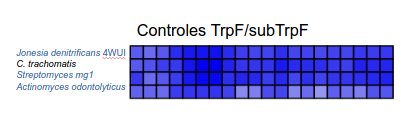
\includegraphics[angle = 0,scale = 0.6]{chapter2/TrpFHeatPlot.png}
  \caption[Heat Plot TrpF Streptomyces vs other subtrates]{\normalsize{Heat Plot TrpF Streptomyces vs other subtrates}}
  \label{fig:TrpFDocking}
  \end{figure}
  
  \TeX~is the best way to typeset mathematics. Donald Knuth designed
  \TeX~when he got frustrated at how long it was taking the typesetters to
  finish his book, which contained a lot of mathematics. One nice feature
  of \emph{R Markdown} is its ability to read \LaTeX~code directly.
  
  If you are doing a thesis that will involve lots of math, you will want
  to read the following section which has been commented out. If you're
  not going to use math, skip over or delete this next commented section.
  
  \section{Chemistry 101: Symbols}\label{chemistry-101-symbols}
  
  Chemical formulas will look best if they are not italicized. Get around
  math mode's automatic italicizing in \LaTeX~by using the argument
  \texttt{\$\textbackslash{}mathrm\{formula\ here\}\$}, with your formula
  inside the curly brackets. (Notice the use of the backticks here which
  enclose text that acts as code.)
  
  So, \(\mathrm{Fe_2^{2+}Cr_2O_4}\) is written
  \texttt{\$\textbackslash{}mathrm\{Fe\_2\^{}\{2+\}Cr\_2O\_4\}\$}.
  
  \noindent Exponent or Superscript: \(\mathrm{O^-}\)
  
  \noindent Subscript: \(\mathrm{CH_4}\)
  
  To stack numbers or letters as in \(\mathrm{Fe_2^{2+}}\), the subscript
  is defined first, and then the superscript is defined.
  
  \noindent Angstrom: \({\AA}\)
  
  \noindent Bullet: CuCl \(\bullet\) \(\mathrm{7H_{2}O}\)
  
  \noindent Double Dagger: \(\ddag\)
  
  \noindent Delta: \(\Delta\)
  
  \noindent Reaction Arrows: \(\longrightarrow\) or
  \(\xrightarrow{solution}\)
  
  \noindent Resonance Arrows: \(\leftrightarrow\)
  
  \noindent Reversible Reaction Arrows: \(\rightleftharpoons\) or
  \(\xrightleftharpoons[ ]{solution}\) (the latter requires the
  \texttt{chemarr} \LaTeX~package which is automatically loaded in this
  template)
  
  \subsection{Typesetting reactions}\label{typesetting-reactions}
  
  You may wish to put your reaction in a figure environment, which means
  that \LaTeX~will place the reaction where it fits and you can have a
  figure caption. You'll see further description of this \textbf{R}
  \texttt{label} function in \protect\hyperlink{refux5flabels}{}. (Note
  the use of the double backslash here as well as the
  \texttt{echo\ =\ FALSE} which hides the code from the output.)
  
  \begin{figure}[h!tbp]
  \begin{center}
  $\mathrm{C_6H_{12}O_6  + 6O_2} \longrightarrow \mathrm{6CO_2 + 6H_2O}$
  \caption{Combustion of glucose}
  \label{fig:comb-gluc}
  \end{center}
  \end{figure}
  
  \subsection{Other examples of
  reactions}\label{other-examples-of-reactions}
  
  \(\mathrm{NH_4Cl_{(s)}}\) \(\rightleftharpoons\)
  \(\mathrm{NH_{3(g)}+HCl_{(g)}}\)
  
  \noindent \(\mathrm{MeCH_2Br + Mg}\) \(\xrightarrow[below]{above}\)
  \(\mathrm{MeCH_2\bullet Mg \bullet Br}\)
  
  \section{Physics}\label{physics}
  
  Many of the symbols you will need can be found on the math page
  \url{http://web.reed.edu/cis/help/latex/math.html} and the Comprehensive
  \LaTeX~Symbol Guide
  (\url{http://mirror.utexas.edu/ctan/info/symbols/comprehensive/symbols-letter.pdf}).
  
  \section{Biology}\label{biology}
  
  You will probably find the resources at
  \url{http://www.lecb.ncifcrf.gov/~toms/latex.html} helpful, particularly
  the links to bsts for various journals. You may also be interested in
  TeXShade for nucleotide typesetting
  (\url{http://homepages.uni-tuebingen.de/beitz/txe.html}). Be sure to
  read the proceeding chapter on graphics and tables.
  
  \chapter{\texorpdfstring{\texttt{\{r\ chapter3,\ child\ =\ \textquotesingle{}chap3.Rmd\textquotesingle{}\}\ \#}}{\{r chapter3, child = 'chap3.Rmd'\} \#}}\label{r-chapter3-child-chap3.rmd}
  
  \chapter{\texorpdfstring{\texttt{\{r\ chapter4,\ child\ =\ \textquotesingle{}chap4.Rmd\textquotesingle{}\}\ \#}}{\{r chapter4, child = 'chap4.Rmd'\} \#}}\label{r-chapter4-child-chap4.rmd}
  
  \chapter{\texorpdfstring{\texttt{\{r\ chapter5,\ child\ =\ \textquotesingle{}chap5.Rmd\textquotesingle{}\}}}{\{r chapter5, child = 'chap5.Rmd'\}}}\label{r-chapter5-child-chap5.rmd}
  
  \chapter*{Conclusion}\label{conclusion}
  \addcontentsline{toc}{chapter}{Conclusion}
  
  \setcounter{chapter}{4} \setcounter{section}{0}
  
  Idea de Rosario -ver dell cluster de saxitoxin cuantos pasos se
  necesitron para llegar ahi.\\
  -A donde se iria el resultado de abrir el GMP\\
  -Otra vez, que Actinos tienen FolE
  
  If we don't want Conclusion to have a chapter number next to it, we can
  add the \texttt{\{.unnumbered\}} attribute. This has an unintended
  consequence of the sections being labeled as 3.6 for example though
  instead of 4.1. The \LaTeX~commands immediately following the Conclusion
  declaration get things back on track.
  
  \subsubsection{More info}\label{more-info}
  
  And here's some other random info: the first paragraph after a chapter
  title or section head \emph{shouldn't be} indented, because indents are
  to tell the reader that you're starting a new paragraph. Since that's
  obvious after a chapter or section title, proper typesetting doesn't add
  an indent there.
  
  \appendix
  
  \chapter{The First Appendix}\label{the-first-appendix}
  
  This first appendix includes all of the R chunks of code that were
  hidden throughout the document (using the \texttt{include\ =\ FALSE}
  chunk tag) to help with readibility and/or setup.
  
  \subsubsection{In the main Rmd file:}\label{in-the-main-rmd-file}
  
  \begin{Shaded}
  \begin{Highlighting}[]
  \CommentTok{# This chunk ensures that the reedtemplates package is}
  \CommentTok{# installed and loaded. This reedtemplates package includes}
  \CommentTok{# the template files for the thesis and also two functions}
  \CommentTok{# used for labeling and referencing}
  \NormalTok{if(!}\KeywordTok{require}\NormalTok{(devtools))}
    \KeywordTok{install.packages}\NormalTok{(}\StringTok{"devtools"}\NormalTok{, }\DataTypeTok{repos =} \StringTok{"http://cran.rstudio.com"}\NormalTok{)}
  \NormalTok{if(!}\KeywordTok{require}\NormalTok{(reedtemplates))\{}
    \KeywordTok{library}\NormalTok{(devtools)}
    \NormalTok{devtools::}\KeywordTok{install_github}\NormalTok{(}\StringTok{"ismayc/reedtemplates"}\NormalTok{)}
  \NormalTok{\}}
  \KeywordTok{library}\NormalTok{(reedtemplates)}
  \end{Highlighting}
  \end{Shaded}
  
  \subsubsection{\texorpdfstring{In
  \protect\hyperlink{refux5flabels}{}:}{In :}}\label{in}
  
  \chapter{The Second Appendix, Open source code on this
  document}\label{the-second-appendix-open-source-code-on-this-document}
  
  \section{R markdown}\label{r-markdown}
  
  Thanks to Rmakdown Thesis\\
  Apendix one Useful docker commands\\
  -Create a new repository\\
  \texttt{docker\ build\ .\ -t\ evomining}\\
  \texttt{docker\ push\ nselemevomining}
  
  \section{Docker}\label{docker}
  
  Reinicie docker para liberar puertos\\
  \texttt{sudo\ service\ docker\ restart}\\
  \texttt{docker\ stop\ \$(docker\ ps\ -a\ -q)}
  
  Detener todos los contenedores
  \texttt{docker\ rm\ \$(docker\ ps\ -a\ -q)}
  
  Remover contenedores detenidos
  \texttt{docker\ rm\ \$(docker\ ps\ -q\ -f\ status=exited)}
  
  Remove all images \texttt{docker\ rmi\ \$(docker\ images\ -q)}
  
  Gblocks only runs inside folder /var/www/html/EvoMining
  
  lista contenedores\\
  \texttt{docker\ ps\ -a}
  
  uninstall docker from ubuntu (Fresh start)\\
  \texttt{sudo\ apt-get\ purge\ docker-engine}\\
  \texttt{sudo\ apt-get\ autoremove\ -\/-purge\ docker-engine}\\
  \texttt{rm\ -rf\ /var/lib/docker} \# This deletes all images,
  containers, and volumes
  
  \texttt{docker\ run\ -i\ -t\ -v\ /home/nelly/GIT/EvoMining/:/var/www/html\ -p\ 80:80\ newevomining\ /bin/bash}
  \texttt{perl\ startevomining}
  
  \section{Git}\label{git}
  
  \texttt{git\ add\ -\/-all} \texttt{git\ commit\ -m\ "Some\ message"}\\
  \texttt{git\ push\ -u\ origin\ master}\\
  \texttt{git\ clone}
  
  \section{Connect GitHub and
  DockerHub}\label{connect-github-and-dockerhub}
  
  automated builds The Dockerfile is available to anyone with access to
  your Docker Hub repository. Your repository is kept up-to-date with code
  changes automatically.
  
  \section{Additional resources}\label{additional-resources}
  
  \begin{itemize}
  \item
    \emph{Markdown} Cheatsheet -
    \url{https://github.com/adam-p/markdown-here/wiki/Markdown-Cheatsheet}
  \item
    \emph{R Markdown} Reference Guide -
    \url{https://www.rstudio.com/wp-content/uploads/2015/03/rmarkdown-reference.pdf}
  \item
    Introduction to \texttt{dplyr} -
    \url{https://cran.rstudio.com/web/packages/dplyr/vignettes/introduction.html}
  \item
    \texttt{ggplot2} Documentation -
    \url{http://docs.ggplot2.org/current/}
  \end{itemize}
  
  \backmatter
  
  \chapter{References}\label{references}
  
  \noindent
  
  \setlength{\parindent}{-0.20in} \setlength{\leftskip}{0.20in}
  \setlength{\parskip}{8pt}
  
  \hypertarget{refs}{}
  \hypertarget{ref-adamsux5fpromiscuousux5f2014}{}
  Adams, N. E., Thiaville, J. J., Proestos, J., Juárez-Vázquez, A. L.,
  McCoy, A. J., Barona-Gómez, F., \ldots{} Maurelli, A. T. (2014).
  Promiscuous and Adaptable Enzymes Fill ``Holes'' in the Tetrahydrofolate
  Pathway in Chlamydia Species. \emph{MBio}, \emph{5}(4).
  \url{http://doi.org/10.1128/mBio.01378-14}
  
  \hypertarget{ref-aharoniux5fevolvabilityux5f2005}{}
  Aharoni, A., Gaidukov, L., Khersonsky, O., Gould, S. M., Roodveldt, C.,
  \& Tawfik, D. S. (2005). The 'evolvability' of promiscuous protein
  functions. \emph{Nature Genetics}, \emph{37}(1), 73--76.
  \url{http://doi.org/10.1038/ng1482}
  
  \hypertarget{ref-angel2000}{}
  Angel, E. (2000). \emph{Interactive computer graphics : A top-down
  approach with openGL}. Boston, MA: Addison Wesley Longman.
  
  \hypertarget{ref-angel2001}{}
  Angel, E. (2001a). \emph{Batch-file computer graphics : A bottom-up
  approach with quickTime}. Boston, MA: Wesley Addison Longman.
  
  \hypertarget{ref-angel2002a}{}
  Angel, E. (2001b). \emph{Test second book by angel}. Boston, MA: Wesley
  Addison Longman.
  
  \hypertarget{ref-azizux5frastux5f2008}{}
  Aziz, R. K., Bartels, D., Best, A. A., DeJongh, M., Disz, T., Edwards,
  R. A., \ldots{} Zagnitko, O. (2008). The RAST Server: Rapid Annotations
  using Subsystems Technology. \emph{BMC Genomics}, \emph{9}, 75.
  \url{http://doi.org/10.1186/1471-2164-9-75}
  
  \hypertarget{ref-baierux5fevolutionux5f2016}{}
  Baier, F., Copp, J. N., \& Tokuriki, N. (2016). Evolution of Enzyme
  Superfamilies: Comprehensive Exploration of Sequence--Function
  Relationships. \emph{Biochemistry}, \emph{55}(46), 6375--6388.
  \url{http://doi.org/10.1021/acs.biochem.6b00723}
  
  \hypertarget{ref-baronagomezux5foccurrenceux5f2003}{}
  Barona Gómez, F., \& Hodgson, D. A. (2003). Occurrence of a putative
  ancient like isomerase involved in histidine and tryptophan
  biosynthesis. \emph{EMBO Reports}, \emph{4}(3), 296--300.
  \url{http://doi.org/10.1038/sj.embor.embor771}
  
  \hypertarget{ref-barona-gomezux5fwhatux5f2012}{}
  Barona-Gómez, F., Cruz-Morales, P., \& Noda-García, L. (2012). What can
  genome-scale metabolic network reconstructions do for prokaryotic
  systematics? \emph{Antonie van Leeuwenhoek}, \emph{101}(1), 35--43.
  \url{http://doi.org/10.1007/s10482-011-9655-1}
  
  \hypertarget{ref-bloomux5fneutralux5f2007}{}
  Bloom, J. D., Romero, P. A., Lu, Z., \& Arnold, F. H. (2007). Neutral
  genetic drift can alter promiscuous protein functions, potentially
  aiding functional evolution. \emph{Biology Direct}, \emph{2}, 17.
  \url{http://doi.org/10.1186/1745-6150-2-17}
  
  \hypertarget{ref-brettinux5frasttk:ux5f2015}{}
  Brettin, T., Davis, J. J., Disz, T., Edwards, R. A., Gerdes, S., Olsen,
  G. J., \ldots{} Xia, F. (2015). RASTtk: A modular and extensible
  implementation of the RAST algorithm for building custom annotation
  pipelines and annotating batches of genomes. \emph{Scientific Reports},
  \emph{5}, 8365. \url{http://doi.org/10.1038/srep08365}
  
  \hypertarget{ref-carbonellux5fmolecularux5f2010}{}
  Carbonell, P., \& Faulon, J.-L. (2010). Molecular signatures-based
  prediction of enzyme promiscuity. \emph{Bioinformatics}, \emph{26}(16),
  2012--2019. \url{http://doi.org/10.1093/bioinformatics/btq317}
  
  \hypertarget{ref-chengux5fglobalux5f2012}{}
  Cheng, X.-Y., Huang, W.-J., Hu, S.-C., Zhang, H.-L., Wang, H., Zhang,
  J.-X., \ldots{} Ji, Z.-L. (2012). A Global Characterization and
  Identification of Multifunctional Enzymes. \emph{PLoS ONE}, \emph{7}(6).
  \url{http://doi.org/10.1371/journal.pone.0038979}
  
  \hypertarget{ref-chesterismayux5fupdatedux5f2016}{}
  chesterismay. (2016, September). Updated R Markdown thesis template.
  \emph{Chester's R blog}. Retrieved from
  \url{https://chesterismay.wordpress.com/2016/09/01/updated-r-markdown-thesis-template/}
  
  \hypertarget{ref-copleyux5fenzymesux5f2003}{}
  Copley, S. D. (2003). Enzymes with extra talents: Moonlighting functions
  and catalytic promiscuity. \emph{Current Opinion in Chemical Biology},
  \emph{7}(2), 265--272.
  \url{http://doi.org/10.1016/S1367-5931(03)00032-2}
  
  \hypertarget{ref-cruz-moralesux5fphylogenomicux5f2016}{}
  Cruz-Morales, P., Kopp, J. F., Martínez-Guerrero, C., Yáñez-Guerra, L.
  A., Selem-Mojica, N., Ramos-Aboites, H., \ldots{} Barona-Gómez, F.
  (2016). Phylogenomic Analysis of Natural Products Biosynthetic Gene
  Clusters Allows Discovery of Arseno-Organic Metabolites in Model
  Streptomycetes. \emph{Genome Biology and Evolution}, \emph{8}(6),
  1906--1916. \url{http://doi.org/10.1093/gbe/evw125}
  
  \hypertarget{ref-deanux5fmechanisticux5f2007}{}
  Dean, A. M., \& Thornton, J. W. (2007). Mechanistic approaches to the
  study of evolution. \emph{Nature Reviews. Genetics}, \emph{8}(9),
  675--688. \url{http://doi.org/10.1038/nrg2160}
  
  \hypertarget{ref-vonux5feichbornux5fpromiscuous:ux5f2011}{}
  Eichborn, J. von, Murgueitio, M. S., Dunkel, M., Koerner, S., Bourne, P.
  E., \& Preissner, R. (2011). PROMISCUOUS: A database for network-based
  drug-repositioning. \emph{Nucleic Acids Research}, \emph{39}(suppl\_1),
  D1060--D1066. \url{http://doi.org/10.1093/nar/gkq1037}
  
  \hypertarget{ref-firnux5fdarwinianux5f2009}{}
  Firn, R. D., \& Jones, C. G. (2009). A Darwinian view of metabolism:
  Molecular properties determine fitness. \emph{Journal of Experimental
  Botany}, \emph{60}(3), 719--726. \url{http://doi.org/10.1093/jxb/erp002}
  
  \hypertarget{ref-garcia-seisdedosux5fprobingux5f2012}{}
  Garcia-Seisdedos, H., Ibarra-Molero, B., \& Sanchez-Ruiz, J. M. (2012).
  Probing the Mutational Interplay between Primary and Promiscuous Protein
  Functions: A Computational-Experimental Approach. \emph{PLOS
  Computational Biology}, \emph{8}(6), e1002558.
  \url{http://doi.org/10.1371/journal.pcbi.1002558}
  
  \hypertarget{ref-glasnerux5fevolutionux5f2006}{}
  Glasner, M. E., Gerlt, J. A., \& Babbitt, P. C. (2006). Evolution of
  enzyme superfamilies. \emph{Current Opinion in Chemical Biology},
  \emph{10}(5), 492--497. \url{http://doi.org/10.1016/j.cbpa.2006.08.012}
  
  \hypertarget{ref-halachevux5fcalculatingux5f2011}{}
  Halachev, M. R., Loman, N. J., \& Pallen, M. J. (2011). Calculating
  Orthologs in Bacteria and Archaea: A Divide and Conquer Approach.
  \emph{PLOS ONE}, \emph{6}(12), e28388.
  \url{http://doi.org/10.1371/journal.pone.0028388}
  
  \hypertarget{ref-hopkinsux5fdrugux5f2009}{}
  Hopkins, A. L. (2009). Drug discovery: Predicting promiscuity.
  \emph{Nature}, \emph{462}(7270), 167--168.
  \url{http://doi.org/10.1038/462167a}
  
  \hypertarget{ref-hughesux5fevolutionux5f1994}{}
  Hughes, A. L. (1994). The Evolution of Functionally Novel Proteins after
  Gene Duplication. \emph{Proceedings of the Royal Society of London B:
  Biological Sciences}, \emph{256}(1346), 119--124.
  \url{http://doi.org/10.1098/rspb.1994.0058}
  
  \hypertarget{ref-hultux5fenzymeux5f2007}{}
  Hult, K., \& Berglund, P. (2007). Enzyme promiscuity: Mechanism and
  applications. \emph{Trends in Biotechnology}, \emph{25}(5), 231--238.
  \url{http://doi.org/10.1016/j.tibtech.2007.03.002}
  
  \hypertarget{ref-jensenux5fenzymeux5f1976}{}
  Jensen. (1976). Enzyme Recruitment in Evolution of New Function.
  \emph{Annual Review of Microbiology}, \emph{30}(1), 409--425.
  \url{http://doi.org/10.1146/annurev.mi.30.100176.002205}
  
  \hypertarget{ref-jiaux5fmultifunctionalux5f2013}{}
  Jia, B., Cheong, G.-W., \& Zhang, S. (2013). Multifunctional enzymes in
  archaea: Promiscuity and moonlight. \emph{Extremophiles}, \emph{17}(2),
  193--203. \url{http://doi.org/10.1007/s00792-012-0509-1}
  
  \hypertarget{ref-khanalux5fdifferentialux5f2015}{}
  Khanal, A., Yu McLoughlin, S., Kershner, J. P., \& Copley, S. D. (2015).
  Differential Effects of a Mutation on the Normal and Promiscuous
  Activities of Orthologs: Implications for Natural and Directed
  Evolution. \emph{Molecular Biology and Evolution}, \emph{32}(1),
  100--108. \url{http://doi.org/10.1093/molbev/msu271}
  
  \hypertarget{ref-khersonskyux5fenzymeux5f2010}{}
  Khersonsky, O., \& Tawfik, D. S. (2010). Enzyme promiscuity: A
  mechanistic and evolutionary perspective. \emph{Annual Review of
  Biochemistry}, \emph{79}, 471--505.
  \url{http://doi.org/10.1146/annurev-biochem-030409-143718}
  
  \hypertarget{ref-kislyukux5fgenomicux5f2011}{}
  Kislyuk, A. O., Haegeman, B., Bergman, N. H., \& Weitz, J. S. (2011).
  Genomic fluidity: An integrative view of gene diversity within microbial
  populations. \emph{BMC Genomics}, \emph{12}, 32.
  \url{http://doi.org/10.1186/1471-2164-12-32}
  
  \hypertarget{ref-kooninux5fturbulentux5f2015}{}
  Koonin, E. V. (2015). The Turbulent Network Dynamics of Microbial
  Evolution and the Statistical Tree of Life. \emph{Journal of Molecular
  Evolution}, \emph{80}(5-6), 244--250.
  \url{http://doi.org/10.1007/s00239-015-9679-7}
  
  \hypertarget{ref-kumariux5fpreparationux5f2007}{}
  Kumari, V., Shah, S., \& Gupta, M. N. (2007). Preparation of Biodiesel
  by Lipase-Catalyzed Transesterification of High Free Fatty Acid
  Containing Oil from Madhuca indica. \emph{Energy \& Fuels},
  \emph{21}(1), 368--372. \url{http://doi.org/10.1021/ef0602168}
  
  \hypertarget{ref-liux5fcomputationalux5f2004}{}
  Li, C., Henry, C. S., Jankowski, M. D., Ionita, J. A., Hatzimanikatis,
  V., \& Broadbelt, L. J. (2004). Computational discovery of biochemical
  routes to specialty chemicals. \emph{Chemical Engineering Science},
  \emph{59}(22--23), 5051--5060.
  \url{http://doi.org/10.1016/j.ces.2004.09.021}
  
  \hypertarget{ref-linsterux5fmetaboliteux5f2013}{}
  Linster, C. L., Van Schaftingen, E., \& Hanson, A. D. (2013). Metabolite
  damage and its repair or pre-emption. \emph{Nature Chemical Biology},
  \emph{9}(2), 72--80. \url{http://doi.org/10.1038/nchembio.1141}
  
  \hypertarget{ref-maux5funconventionalux5f2013}{}
  Ma, H.-M., Zhou, Q., Tang, Y.-M., Zhang, Z., Chen, Y.-S., He, H.-Y.,
  \ldots{} Tang, G.-L. (2013). Unconventional Origin and Hybrid System for
  Construction of Pyrrolopyrrole Moiety in Kosinostatin Biosynthesis.
  \emph{Chemistry \& Biology}, \emph{20}(6), 796--805.
  \url{http://doi.org/10.1016/j.chembiol.2013.04.013}
  
  \hypertarget{ref-martinez-nunezux5flifestyleux5f2015}{}
  Martínez-Núñez, M. A., Rodríguez-Vázquez, K., \& Pérez-Rueda, E. (2015).
  The lifestyle of prokaryotic organisms influences the repertoire of
  promiscuous enzymes. \emph{Proteins: Structure, Function, and
  Bioinformatics}, \emph{83}(9), 1625--1631.
  \url{http://doi.org/10.1002/prot.24847}
  
  \hypertarget{ref-medemaux5fcomputationalux5f2015}{}
  Medema, M. H., \& Fischbach, M. A. (2015). Computational approaches to
  natural product discovery. \emph{Nature Chemical Biology}, \emph{11}(9),
  639--648. \url{http://doi.org/10.1038/nchembio.1884}
  
  \hypertarget{ref-medemaux5fantismash:ux5f2011}{}
  Medema, M. H., Blin, K., Cimermancic, P., Jager, V. de, Zakrzewski, P.,
  Fischbach, M. A., \ldots{} Breitling, R. (2011). antiSMASH: Rapid
  identification, annotation and analysis of secondary metabolite
  biosynthesis gene clusters in bacterial and fungal genome sequences.
  \emph{Nucleic Acids Research}, \emph{39}(Web Server issue), W339--W346.
  \url{http://doi.org/10.1093/nar/gkr466}
  
  \hypertarget{ref-nagaoux5fpredictionux5f2014}{}
  Nagao, C., Nagano, N., \& Mizuguchi, K. (2014). Prediction of Detailed
  Enzyme Functions and Identification of Specificity Determining Residues
  by Random Forests. \emph{PLOS ONE}, \emph{9}(1), e84623.
  \url{http://doi.org/10.1371/journal.pone.0084623}
  
  \hypertarget{ref-narechaniaux5frandomux5f2012}{}
  Narechania, A., Baker, R. H., Sit, R., Kolokotronis, S.-O., DeSalle, R.,
  \& Planet, P. J. (2012). Random Addition Concatenation Analysis: A Novel
  Approach to the Exploration of Phylogenomic Signal Reveals Strong
  Agreement between Core and Shell Genomic Partitions in the
  Cyanobacteria. \emph{Genome Biology and Evolution}, \emph{4}(1), 30--43.
  \url{http://doi.org/10.1093/gbe/evr121}
  
  \hypertarget{ref-nathux5fquantitativeux5f2008}{}
  Nath, A., \& Atkins, W. M. (2008). A Quantitative Index of Substrate
  Promiscuity. \emph{Biochemistry}, \emph{47}(1), 157--166.
  \url{http://doi.org/10.1021/bi701448p}
  
  \hypertarget{ref-nathux5fquantifyingux5f2010}{}
  Nath, A., Zientek, M. A., Burke, B. J., Jiang, Y., \& Atkins, W. M.
  (2010). Quantifying and Predicting the Promiscuity and Isoform
  Specificity of Small-Molecule Cytochrome P450 Inhibitors. \emph{Drug
  Metabolism and Disposition}, \emph{38}(12), 2195--2203.
  \url{http://doi.org/10.1124/dmd.110.034645}
  
  \hypertarget{ref-nobeliux5fproteinux5f2009}{}
  Nobeli, I., Favia, A. D., \& Thornton, J. M. (2009). Protein promiscuity
  and its implications for biotechnology. \emph{Nature Biotechnology},
  \emph{27}(2), 157--167. \url{http://doi.org/10.1038/nbt1519}
  
  \hypertarget{ref-noda-garciaux5fevolutionux5f2013}{}
  Noda-García, L., Camacho-Zarco, A. R., Medina-Ruíz, S., Gaytán, P.,
  Carrillo-Tripp, M., Fülöp, V., \& Barona-Gómez, F. (2013). Evolution of
  Substrate Specificity in a Recipient's Enzyme Following Horizontal Gene
  Transfer. \emph{Molecular Biology and Evolution}, \emph{30}(9),
  2024--2034. \url{http://doi.org/10.1093/molbev/mst115}
  
  \hypertarget{ref-noda-garciaux5finsightsux5f2015}{}
  Noda-García, L., Juárez-Vázquez, A. L., Ávila-Arcos, M. C.,
  Verduzco-Castro, E. A., Montero-Morán, G., Gaytán, P., \ldots{}
  Barona-Gómez, F. (2015). Insights into the evolution of enzyme substrate
  promiscuity after the discovery of \(\beta\alpha_8\) isomerase
  evolutionary intermediates from a diverse metagenome. \emph{BMC
  Evolutionary Biology}, \emph{15}.
  \url{http://doi.org/10.1186/s12862-015-0378-1}
  
  \hypertarget{ref-notebaartux5fnetwork-levelux5f2014}{}
  Notebaart, R. A., Szappanos, B., Kintses, B., Pál, F., Györkei, Á.,
  Bogos, B., \ldots{} Papp, B. (2014). Network-level architecture and the
  evolutionary potential of underground metabolism. \emph{Proceedings of
  the National Academy of Sciences}, \emph{111}(32), 11762--11767.
  \url{http://doi.org/10.1073/pnas.1406102111}
  
  \hypertarget{ref-overbeekux5fuseux5f1999}{}
  Overbeek, R., Fonstein, M., D'Souza, M., Pusch, G. D., \& Maltsev, N.
  (1999). The use of gene clusters to infer functional coupling.
  \emph{Proceedings of the National Academy of Sciences}, \emph{96}(6),
  2896--2901. \url{http://doi.org/10.1073/pnas.96.6.2896}
  
  \hypertarget{ref-overbeekux5fseedux5f2014}{}
  Overbeek, R., Olson, R., Pusch, G. D., Olsen, G. J., Davis, J. J., Disz,
  T., \ldots{} Stevens, R. (2014). The SEED and the Rapid Annotation of
  microbial genomes using Subsystems Technology (RAST). \emph{Nucleic
  Acids Research}, \emph{42}(Database issue), D206--D214.
  \url{http://doi.org/10.1093/nar/gkt1226}
  
  \hypertarget{ref-obrienux5fcatalyticux5f1999}{}
  O'Brien, P. J., \& Herschlag, D. (1999). Catalytic promiscuity and the
  evolution of new enzymatic activities. \emph{Chemistry \& Biology},
  \emph{6}(4), R91--R105.
  \url{http://doi.org/10.1016/S1074-5521(99)80033-7}
  
  \hypertarget{ref-pandyaux5fenzymeux5f2014}{}
  Pandya, C., Farelli, J. D., Dunaway-Mariano, D., \& Allen, K. N. (2014).
  Enzyme Promiscuity: Engine of Evolutionary Innovation. \emph{Journal of
  Biological Chemistry}, \emph{289}(44), 30229--30236.
  \url{http://doi.org/10.1074/jbc.R114.572990}
  
  \hypertarget{ref-patrickux5fmulticopyux5f2007}{}
  Patrick, W. M., Quandt, E. M., Swartzlander, D. B., \& Matsumura, I.
  (2007). Multicopy Suppression Underpins Metabolic Evolvability.
  \emph{Molecular Biology and Evolution}, \emph{24}(12), 2716--2722.
  \url{http://doi.org/10.1093/molbev/msm204}
  
  \hypertarget{ref-pearsonux5fprehistoricux5f2012}{}
  Pearson, H. (2012). Prehistoric proteins: Raising the dead. \emph{Nature
  News}, \emph{483}(7390), 390. \url{http://doi.org/10.1038/483390a}
  
  \hypertarget{ref-rissoux5fphenotypicux5f2014}{}
  Risso, V. A., Gavira, J. A., Gaucher, E. A., \& Sanchez Ruiz, J. M.
  (2014). Phenotypic comparisons of consensus variants versus laboratory
  resurrections of precambrian proteins. \emph{Proteins: Structure,
  Function, and Bioinformatics}, \emph{82}(6), 887--896.
  \url{http://doi.org/10.1002/prot.24575}
  
  \hypertarget{ref-sanchez-ruizux5fpromiscuityux5f2012}{}
  Sanchez-Ruiz, J. M. (2012). On promiscuity, changing environments and
  the possibility of replaying the molecular tape of life.
  \emph{Biochemical Journal}, \emph{445}(1), e1--e3.
  \url{http://doi.org/10.1042/BJ20120806}
  
  \hypertarget{ref-snelux5fstring:ux5f2000}{}
  Snel, B., Lehmann, G., Bork, P., \& Huynen, M. A. (2000). STRING: A
  web-server to retrieve and display the repeatedly occurring
  neighbourhood of a gene. \emph{Nucleic Acids Research}, \emph{28}(18),
  3442--3444. Retrieved from
  \url{http://www.ncbi.nlm.nih.gov/pmc/articles/PMC110752/}
  
  \hypertarget{ref-soskineux5fmutationalux5f2010}{}
  Soskine, M., \& Tawfik, D. S. (2010). Mutational effects and the
  evolution of new protein functions. \emph{Nature Reviews Genetics},
  \emph{11}(8), 572--582. \url{http://doi.org/10.1038/nrg2808}
  
  \hypertarget{ref-szklarczykux5fstringux5f2015}{}
  Szklarczyk, D., Franceschini, A., Wyder, S., Forslund, K., Heller, D.,
  Huerta-Cepas, J., \ldots{} Mering, C. von. (2015). STRING v10:
  Protein--protein interaction networks, integrated over the tree of life.
  \emph{Nucleic Acids Research}, \emph{43}(D1), D447--D452.
  \url{http://doi.org/10.1093/nar/gku1003}
  
  \hypertarget{ref-treangenux5fhorizontalux5f2011}{}
  Treangen, T. J., \& Rocha, E. P. C. (2011). Horizontal Transfer, Not
  Duplication, Drives the Expansion of Protein Families in Prokaryotes.
  \emph{PLOS Genetics}, \emph{7}(1), e1001284.
  \url{http://doi.org/10.1371/journal.pgen.1001284}
  
  \hypertarget{ref-verdel-arandaux5fmolecularux5f2015}{}
  Verdel-Aranda, K., López-Cortina, S. T., Hodgson, D. A., \&
  Barona-Gómez, F. (2015). Molecular annotation of ketol-acid
  reductoisomerases from Streptomyces reveals a novel amino acid
  biosynthesis interlock mediated by enzyme promiscuity. \emph{Microbial
  Biotechnology}, \emph{8}(2), 239--252.
  \url{http://doi.org/10.1111/1751-7915.12175}
  
  \hypertarget{ref-weberux5fantismashux5f2015}{}
  Weber, T., Blin, K., Duddela, S., Krug, D., Kim, H. U., Bruccoleri, R.,
  \ldots{} Medema, M. H. (2015). antiSMASH 3.0---a comprehensive resource
  for the genome mining of biosynthetic gene clusters. \emph{Nucleic Acids
  Research}, \emph{43}(W1), W237--W243.
  \url{http://doi.org/10.1093/nar/gkv437}
  
  \hypertarget{ref-zhangux5fmultidimensionalux5f2012}{}
  Zhang, W., Dourado, D. F. A. R., Fernandes, P. A., Ramos, M. J., \&
  Mannervik, B. (2012). Multidimensional epistasis and fitness landscapes
  in enzyme evolution. \emph{Biochemical Journal}, \emph{445}(1), 39--46.
  \url{http://doi.org/10.1042/BJ20120136}
  
  \hypertarget{ref-zhaoux5fdiscoveryux5f2013}{}
  Zhao, S., Kumar, R., Sakai, A., Vetting, M. W., Wood, B. M., Brown, S.,
  \ldots{} Jacobson, M. P. (2013). Discovery of new enzymes and metabolic
  pathways by using structure and genome context. \emph{Nature},
  \emph{502}(7473), 698--702. \url{http://doi.org/10.1038/nature12576}
  
  \hypertarget{ref-zhaoux5fpredictionux5f2014}{}
  Zhao, S., Sakai, A., Zhang, X., Vetting, M. W., Kumar, R., Hillerich,
  B., \ldots{} Jacobson, M. P. (2014). Prediction and characterization of
  enzymatic activities guided by sequence similarity and genome
  neighborhood networks. \emph{ELife}, \emph{3}, e03275.
  \url{http://doi.org/10.7554/eLife.03275}
  
  \hypertarget{ref-zouux5fevolutionux5f2015}{}
  Zou, T., Risso, V. A., Gavira, J. A., Sanchez-Ruiz, J. M., \& Ozkan, S.
  B. (2015). Evolution of Conformational Dynamics Determines the
  Conversion of a Promiscuous Generalist into a Specialist Enzyme.
  \emph{Molecular Biology and Evolution}, \emph{32}(1), 132--143.
  \url{http://doi.org/10.1093/molbev/msu281}


  % Index?

\end{document}

